\chapter{The module \pyvisi}
\label{PYVISI CHAP}

\declaremodule{extension}{pyvisi}
\modulesynopsis{Python visualization interface}

\pyvisi provides an easy to use interface to the \VTK visualization 
tool. \pyvisi provides the following modules:

\begin{itemize}
\item \Scene: Shows a scene in which components are to be displayed.
\item \Image: Shows an image.
\item \Text: Shows some 2D text.
\item \DataCollector: Deals with data for visualization.
\item \Camera: Controls the camera manipulation. 
\item \Light: Controls the light manipulation.
\item \Map: Shows a scalar field by color on the domain surface.
\item \MapOnPlane: Shows a scalar field by color on a given plane. 
\item \MapOnClip: Shows a scalar field by color on a given clip.
\item \MapOnScalarClip: Shows a scalar field by color on a give scalar clip.
\item \Arrows: Shows a vector field by arrows.
\item \ArrowsOnPlane: Shows a vector field by arrows on a given plane.
\item \ArrowsOnClip: Shows a vector field by arrows on a given clip.
\item \IsoSurface: Shows a scalar field for a given value by 
an isosurface.
\item \IsoSurfaceOnPlane: Shows a scalar field for a given value by 
an isosurfaceon a given plane.
\item \IsoSurfaceOnClip: Shows a scalar field for a given vlaue by 
an isosurface on a given clip.
\item \Contour: Shows a scalar field by contour surfaces. 
\item \ContourOnPlane: Shows a scalar field by contour surfaces on 
a given plane.
\item \ContourOnClip: Shows a scalar field by contour surfaces on 
a given clip.
\item \TensorC: Shows a tensor field by ellipsoids.
\item \TensorOnPlane: Shows a tensor field by ellipsoids on 
a given plane.
\item \TensorOnClip: Shows a tensor field by ellipsoids on a given clip.
\item \StreamLines: Shows the path of particles in a vector field.
\item \Carpet: Shows a scalar field as plane deformated along 
the plane normal.
\item \Position: Defines the x,y and z coordinates rendered object.
\item \Transform: Defines the orientation of rendered object.
\item \Style: Defines the style of text.
\item \BlueToRed: Defines a map spectrum from blue to red.
\item \RedToBlue: Defines a map spectrum from red to blue.
\item \Plane: Defines the cutting/clipping of rendered objects.
\end{itemize}

\section{\Scene class}
\begin{classdesc}{Scene}{renderer, x_size = 500, y_size = 500}
A \Scene object creates a window onto which objects are to be displayed. 
\end{classdesc}

The following are the methods available:
\begin{methoddesc}[Scene]{saveImage}{image_name}
Save the rendered object as an image off-screen. 
\end{methoddesc}

\begin{methoddesc}[Scene]{render}{}
Render the object on-screen.
\end{methoddesc}

The following is a sample code using the \Scene class:
\verbatiminput{../examples/driverscene.py}

\section{\Image class}
\begin{classdesc}{Image}{scene, format}
An \Image object shows an image.
\end{classdesc}

The following is the method available:
\begin{methoddesc}[Image]{setFileName}{file_name}
Set the file name.
\end{methoddesc}

The following is a sample code using the \Image class.
\fig{fig:image.1} shows the corresponding output.
\verbatiminput{../examples/driverimage.py}

\begin{figure}[ht]
\begin{center}
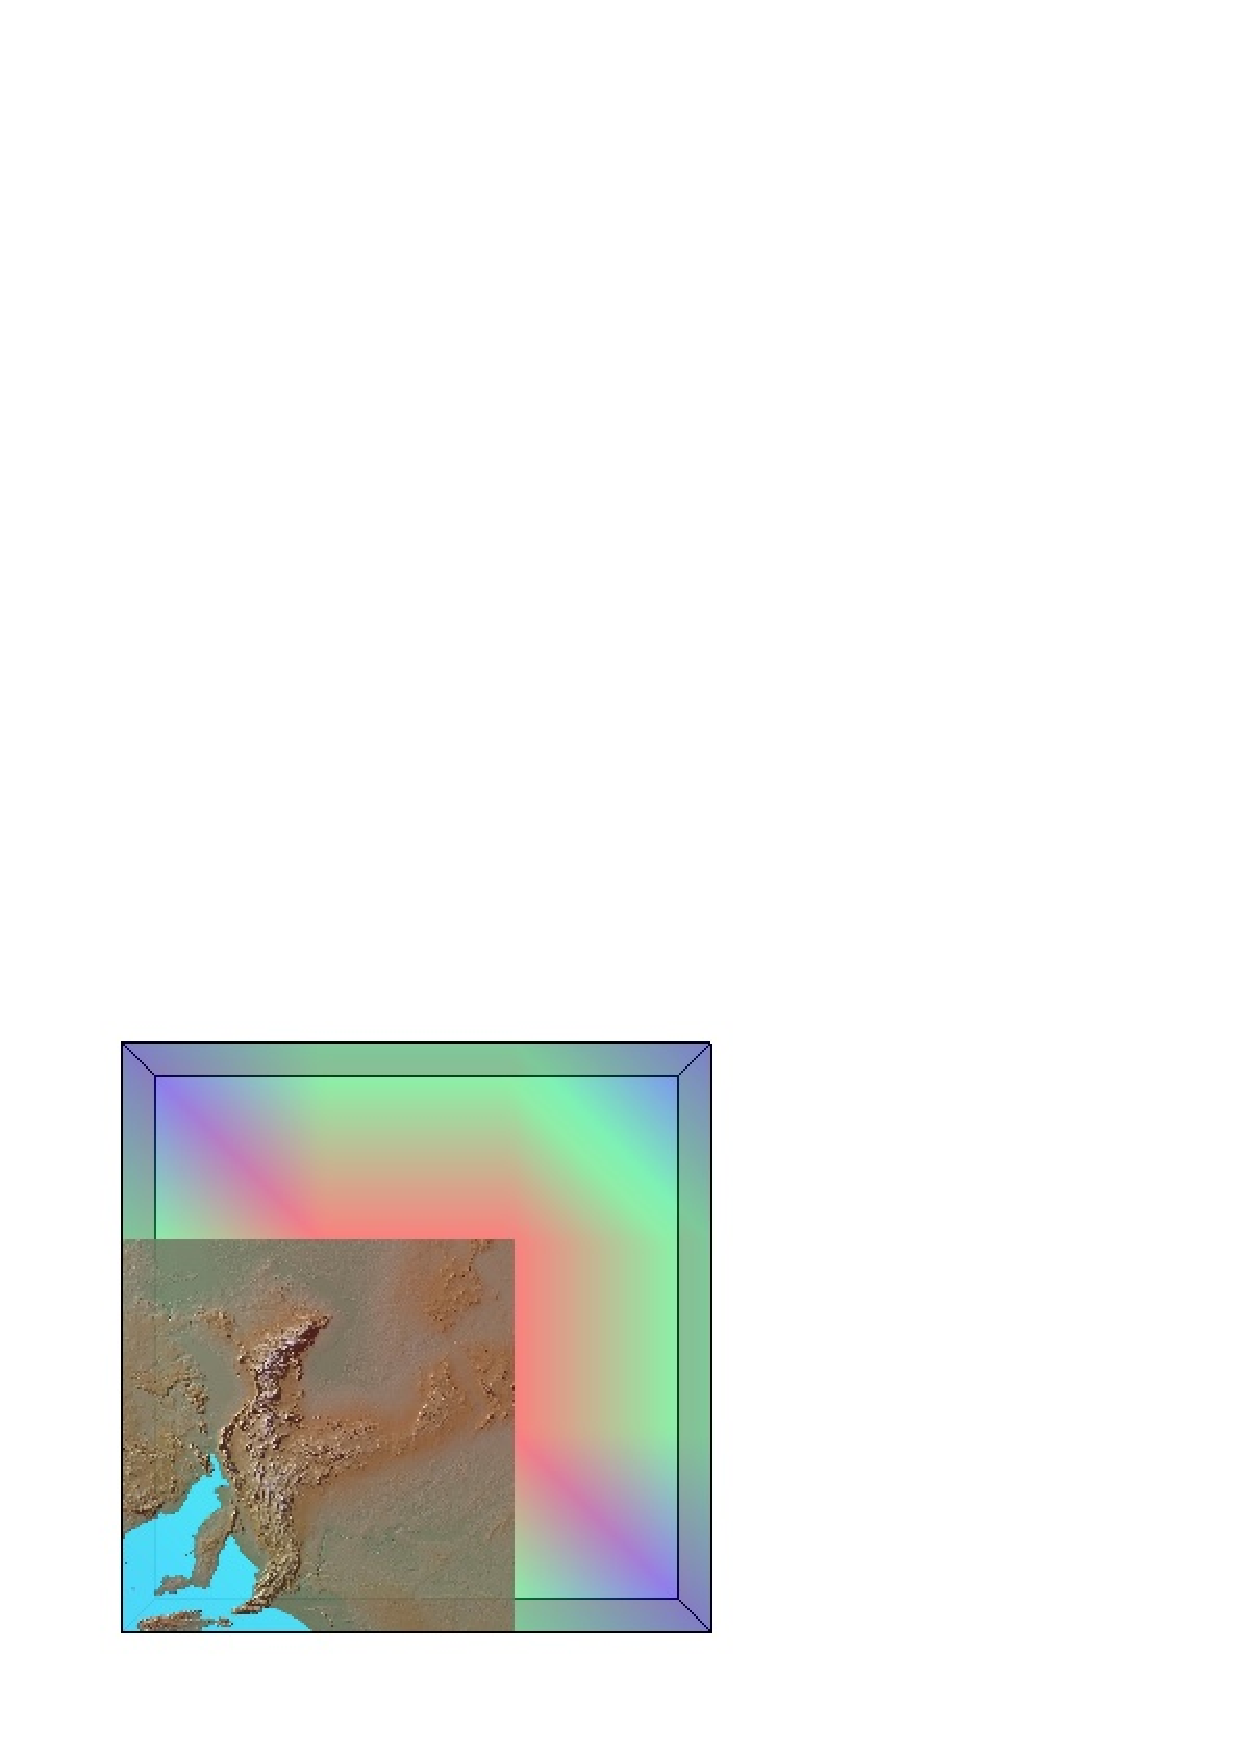
\includegraphics[width=40mm]{figures/Image}
\end{center}
\caption{Image}
\label{fig:image.1}
\end{figure}

\section{\Text class}
\begin{classdesc}{Text}{scene}
A \Text object shows 2D text. 
\end{classdesc}

The following are the methods available:
\begin{methoddesc}[Text]{setText}{text}
Set the text.
\end{methoddesc}

\begin{methoddesc}[Text]{setPosition}{x_coor, y_coor}
Set the display position of the text.
\end{methoddesc}

\begin{methoddesc}[Text]{setStyle}{style}
Set the style of the text.
\end{methoddesc}

The following is a sample code using the \Text class.
\fig{fig:text.1} shows the corresponding output.
\verbatiminput{../examples/drivertext.py}

\begin{figure}[ht]
\begin{center}
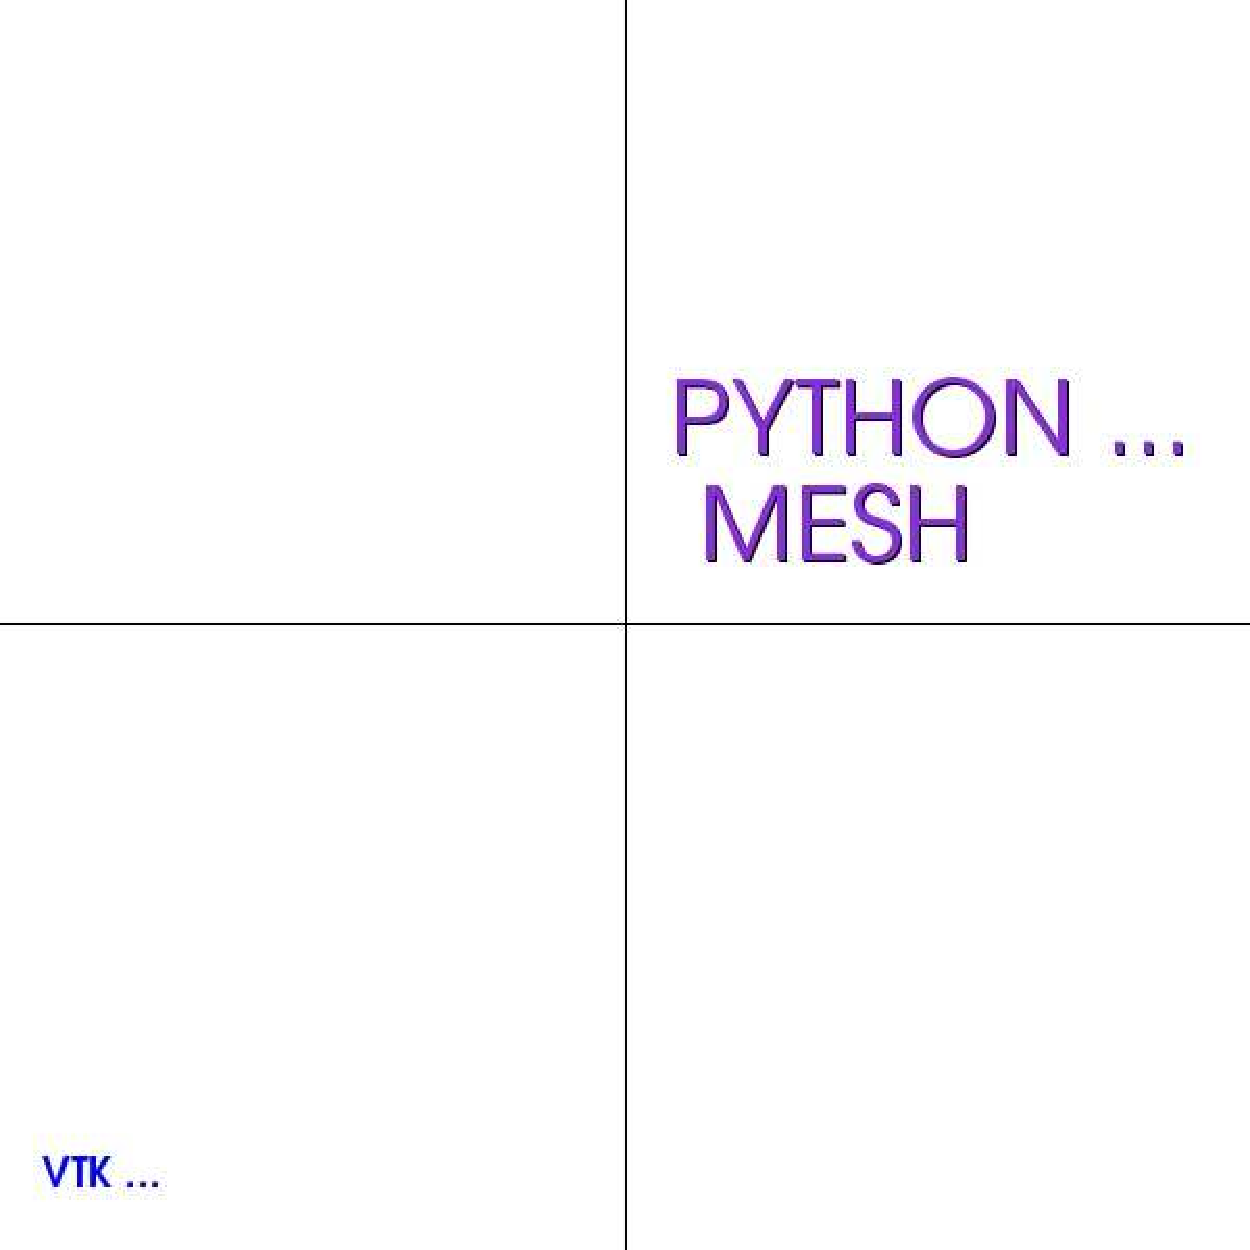
\includegraphics[width=40mm]{figures/Text}
\end{center}
\caption{2D text}
\label{fig:text.1}
\end{figure}

\section{\DataCollector class}
\begin{classdesc}{DataCollector}{scene, outline = True, cube_axes = False}
A \DataCollector object deals with the data for visualization.
\end{classdesc}

The following are the methods available:
\begin{methoddesc}[DataCollector]{setFileName}{file_name}
Set the file name from which data is to be read.
\end{methoddesc}

The following is a sample code using the \DataCollector class. 
\fig{fig:datacollector.1} shows the corresponding output. 
\verbatiminput{../examples/driverdatacollector.py}

\begin{figure}[ht]
\begin{center}
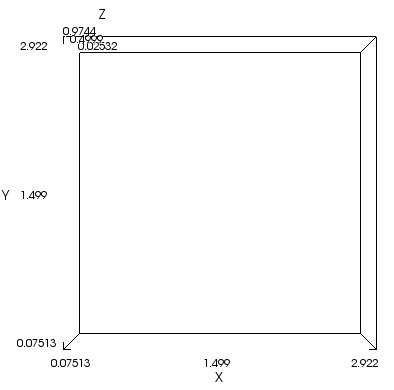
\includegraphics[width=40mm]{figures/DataCollector}
\end{center}
\caption{Datacollector generating an outline with cube axes.}
\label{fig:datacollector.1}
\end{figure}

\section{\Camera class}
\begin{classdesc}{Camera}{scene, data_collector}
A \Camera object controls the camera's settings.
\end{classdesc}

The following are some of the methods available:
\begin{methoddesc}[Camera]{setFocalPoint}{position}
Set the focal point of the camera.
\end{methoddesc}

\begin{methoddesc}[Camera]{setPosition}{position}
Set the position of the camera.
\end{methoddesc}

\begin{methoddesc}[Camera]{azimuth}{angle}
Rotate the camera to the left and right.
\end{methoddesc}

\begin{methoddesc}[Camera]{elevation}{angle}
Rotate the camera to the top and bottom.
\end{methoddesc}

\begin{methoddesc}[Camera]{roll}{angle}
Roll the camera to the left and right.
\end{methoddesc}

\begin{methoddesc}[Camera]{backView}{}
View the back of the rendered object.
\end{methoddesc}

\begin{methoddesc}[Camera]{topView}{}
View the top of the rendered object.
\end{methoddesc}

\begin{methoddesc}[Camera]{bottomView}{}
View the bottom of the rendered object.
\end{methoddesc}

\begin{methoddesc}[Camera]{leftView}{}
View the left side of the rendered object.
\end{methoddesc}

\begin{methoddesc}[Camera]{rightView}{}
View the right side of the rendered object.
\end{methoddesc}

\begin{methoddesc}[Camera]{isometricView}{}
View the isometric side of the rendered object.
\end{methoddesc}

The following is a sample code using the \Camera class. 
\fig{fig:camera.1} shows the corresponding output. 
\verbatiminput{../examples/drivercamera.py}

\begin{figure}[ht]
\begin{center}
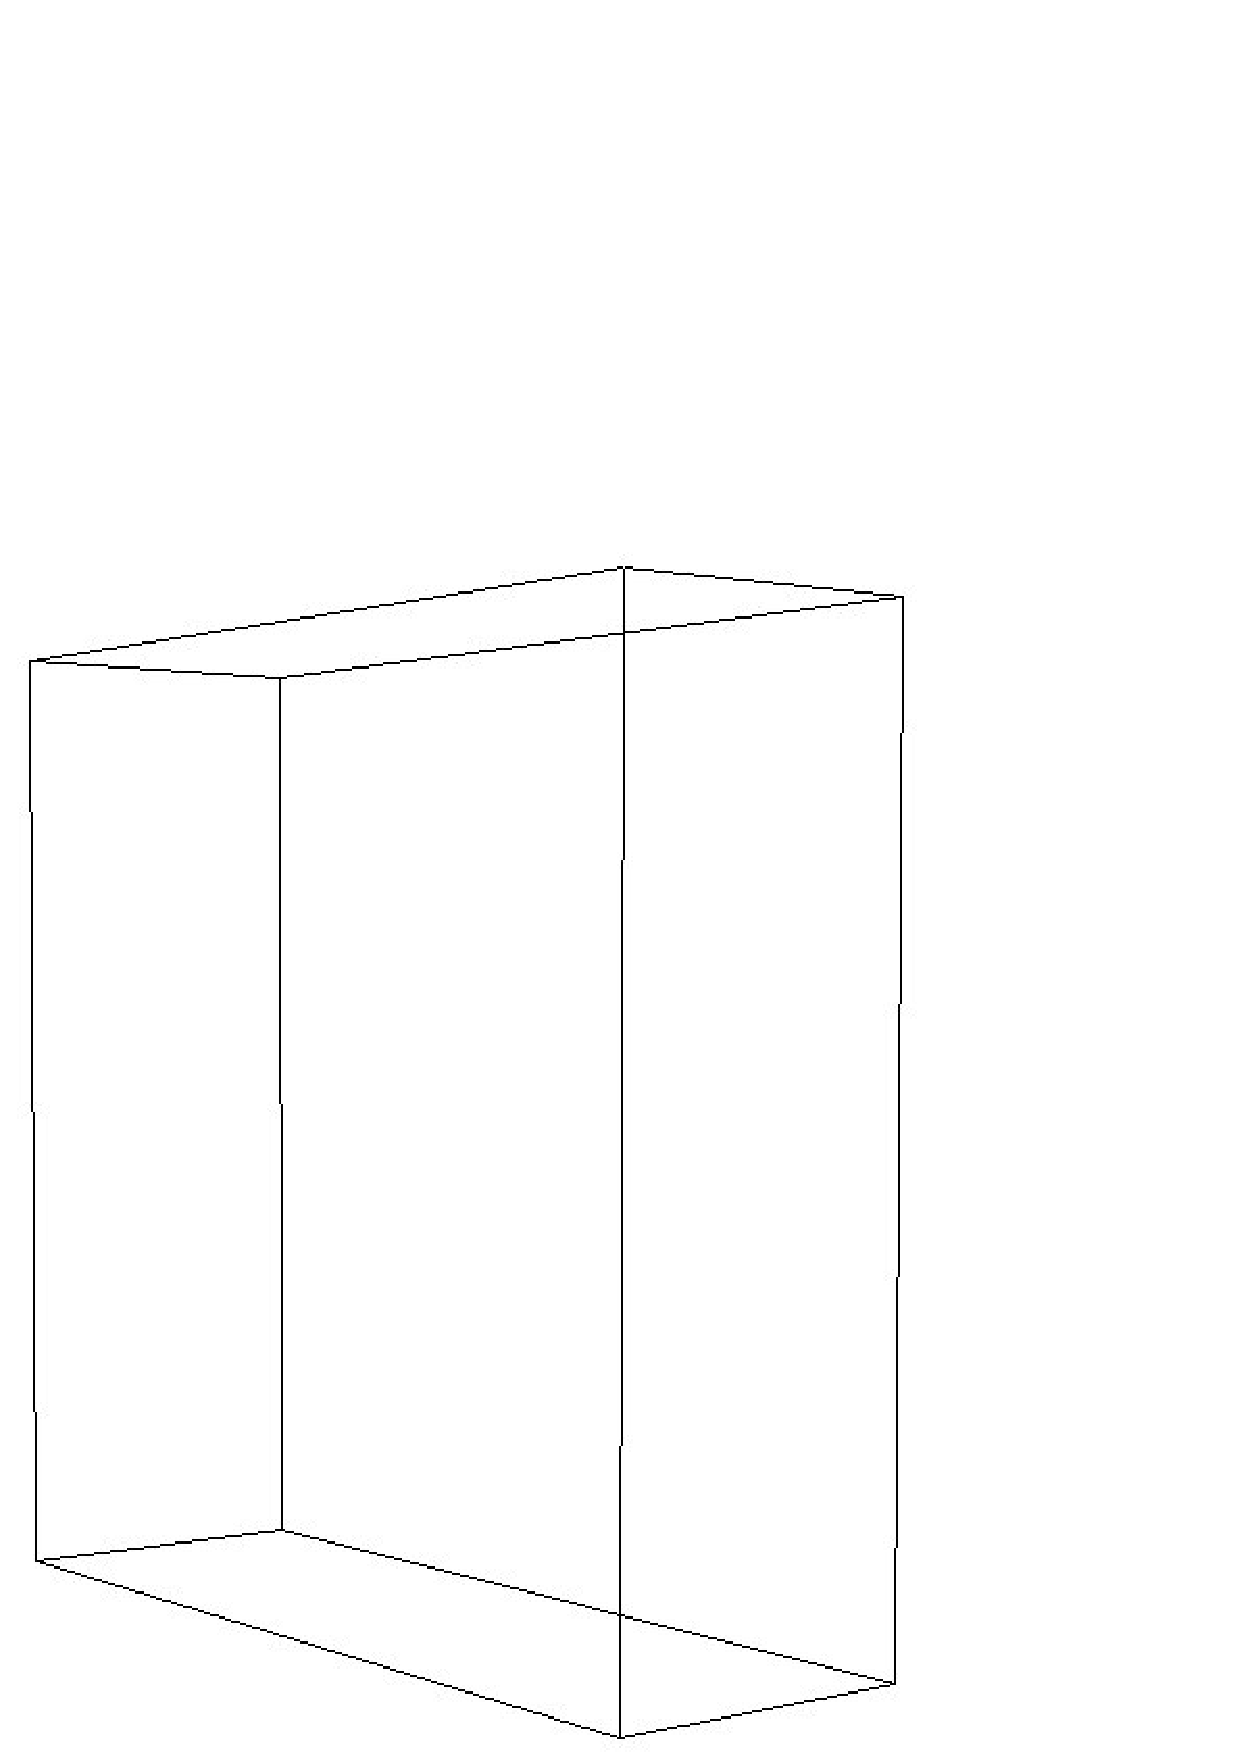
\includegraphics[width=30mm]{figures/Camera}
\end{center}
\caption{Camera manipulation}
\label{fig:camera.1}
\end{figure}

\section{\Light class}
\begin{classdesc}{Light}{scene, data_collector}
A \Light object controls the light's settings. 
\end{classdesc}

The following are the methods available:
\begin{methoddesc}[Light]{setColor}{color}
Set the color of the light.
\end{methoddesc}

\begin{methoddesc}[Light]{setFocalPoint}{position}
Set the focal point of the light.
\end{methoddesc}

\begin{methoddesc}[Light]{setPosition}{position}
Set the position of the light.
\end{methoddesc}

\begin{methoddesc}[Light]{setIntensity}{intesity}
Set the intensity (brightness) of the light.
\end{methoddesc}

The following is a sample code using the \Light class.
\fig{fig:light.1} shows the corresponding output.
\verbatiminput{../examples/driverlight.py}

\begin{figure}[ht]
\begin{center}
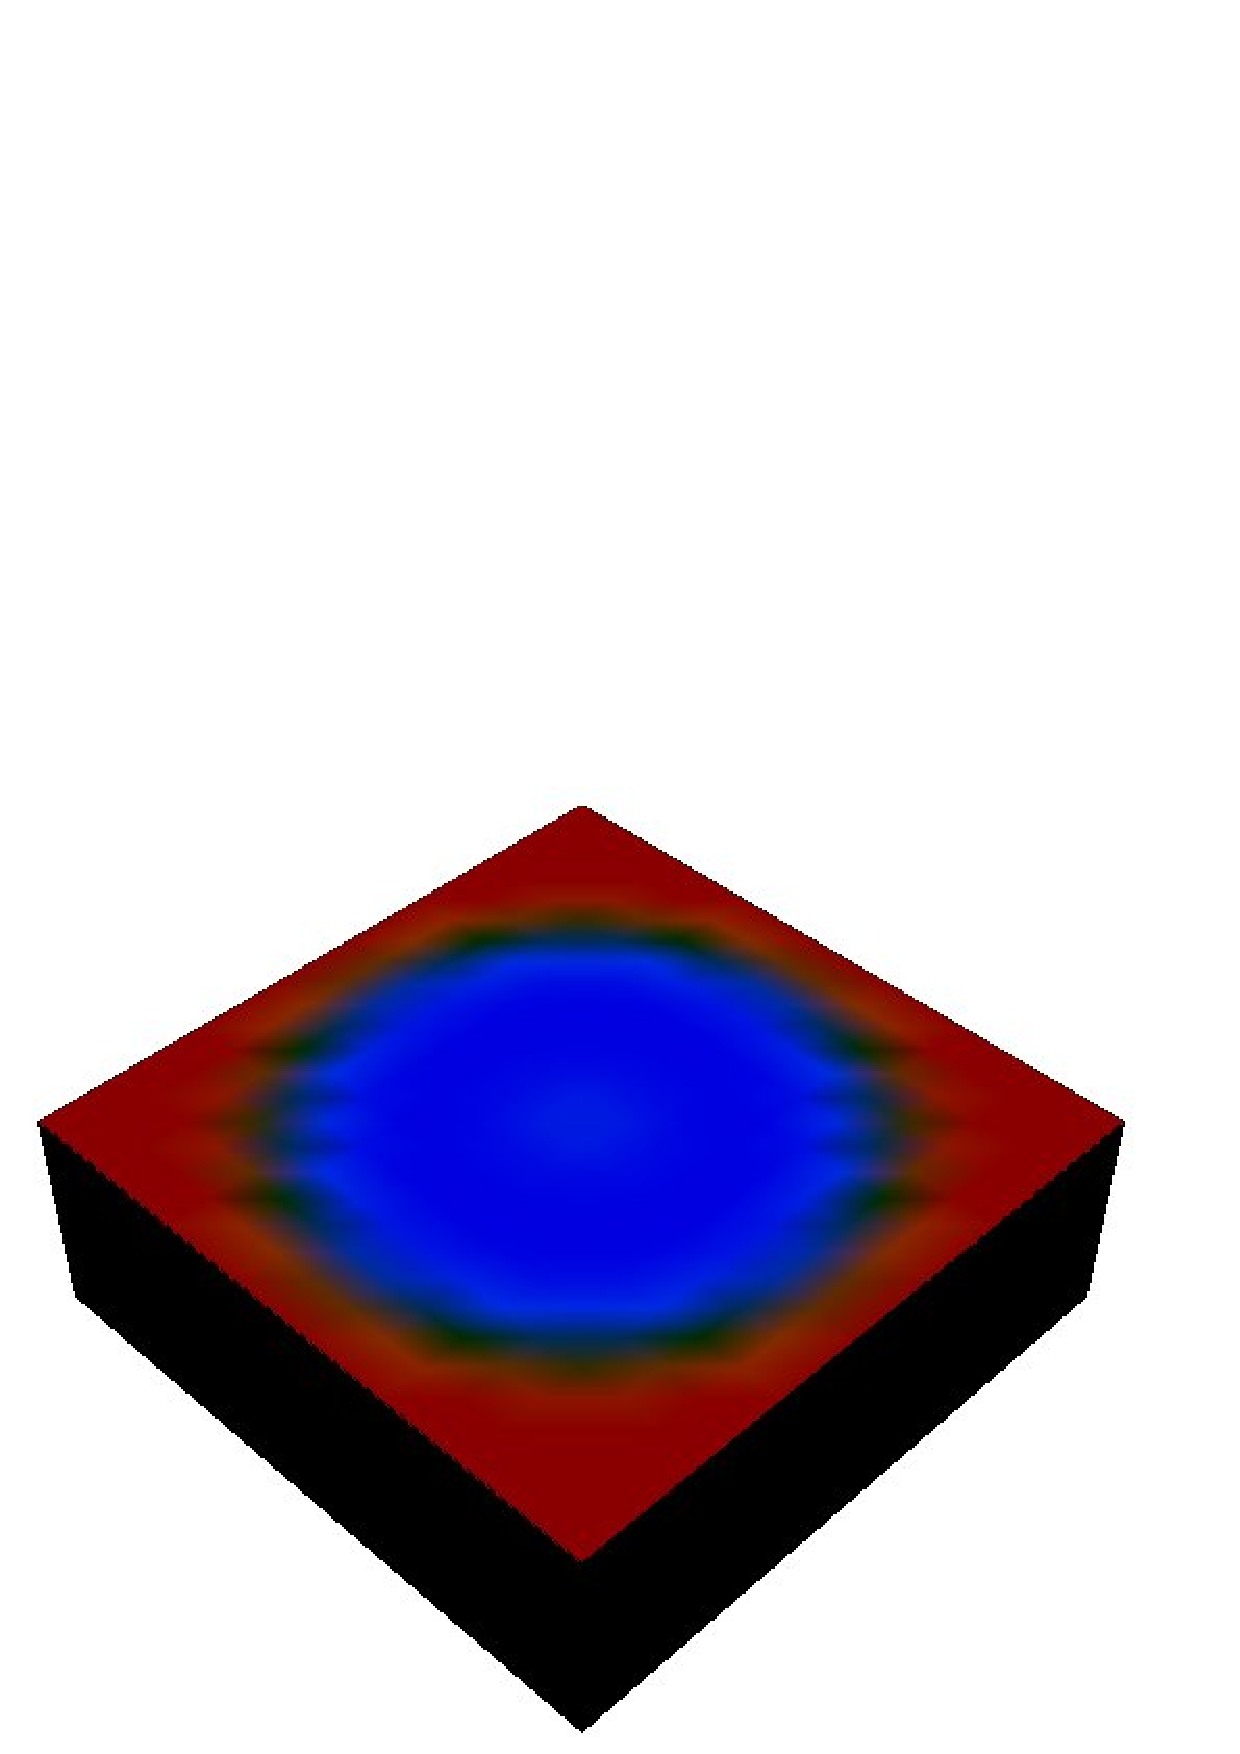
\includegraphics[width=40mm]{figures/Light}
\end{center}
\caption{Light}
\label{fig:light.1}
\end{figure}

\section{\Map class}
\begin{classdesc}{Map}{scene, data_collector, lut = None}
A \Map object shows a scalar field by color on the domain surface.
\end{classdesc}

The following is a sample code using the \Map class. 
\fig{fig:map.1} shows the corresponding output. 
\verbatiminput{../examples/drivermap.py}

\begin{figure}[ht]
\begin{center}
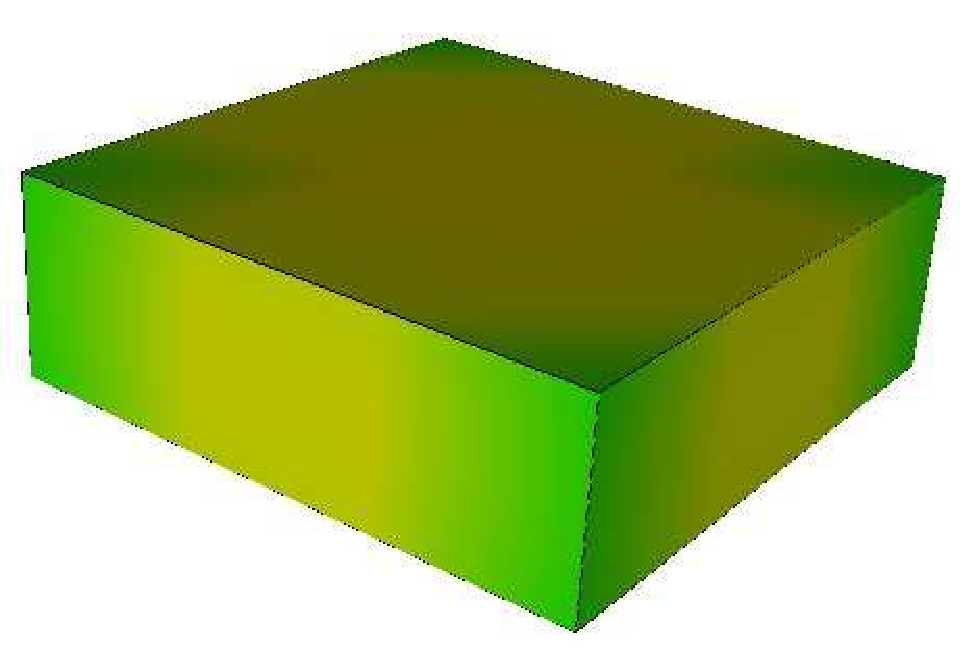
\includegraphics[width=40mm]{figures/Map}
\end{center}
\caption{Surface map}
\label{fig:map.1}
\end{figure}

\section{\MapOnPlane class}
\begin{classdesc}{MapOnPlane}{scene, data_collector, transform, lut = None}
A \MapOnPlane object show a scalar field by color on a given plane.
\end{classdesc}

The following is a sample code using the \MapOnPlane class.
\fig{fig:maponplane.1} shows the corresponding output. 
\verbatiminput{../examples/drivermaponplane.py}

\begin{figure}[ht]
\begin{center}
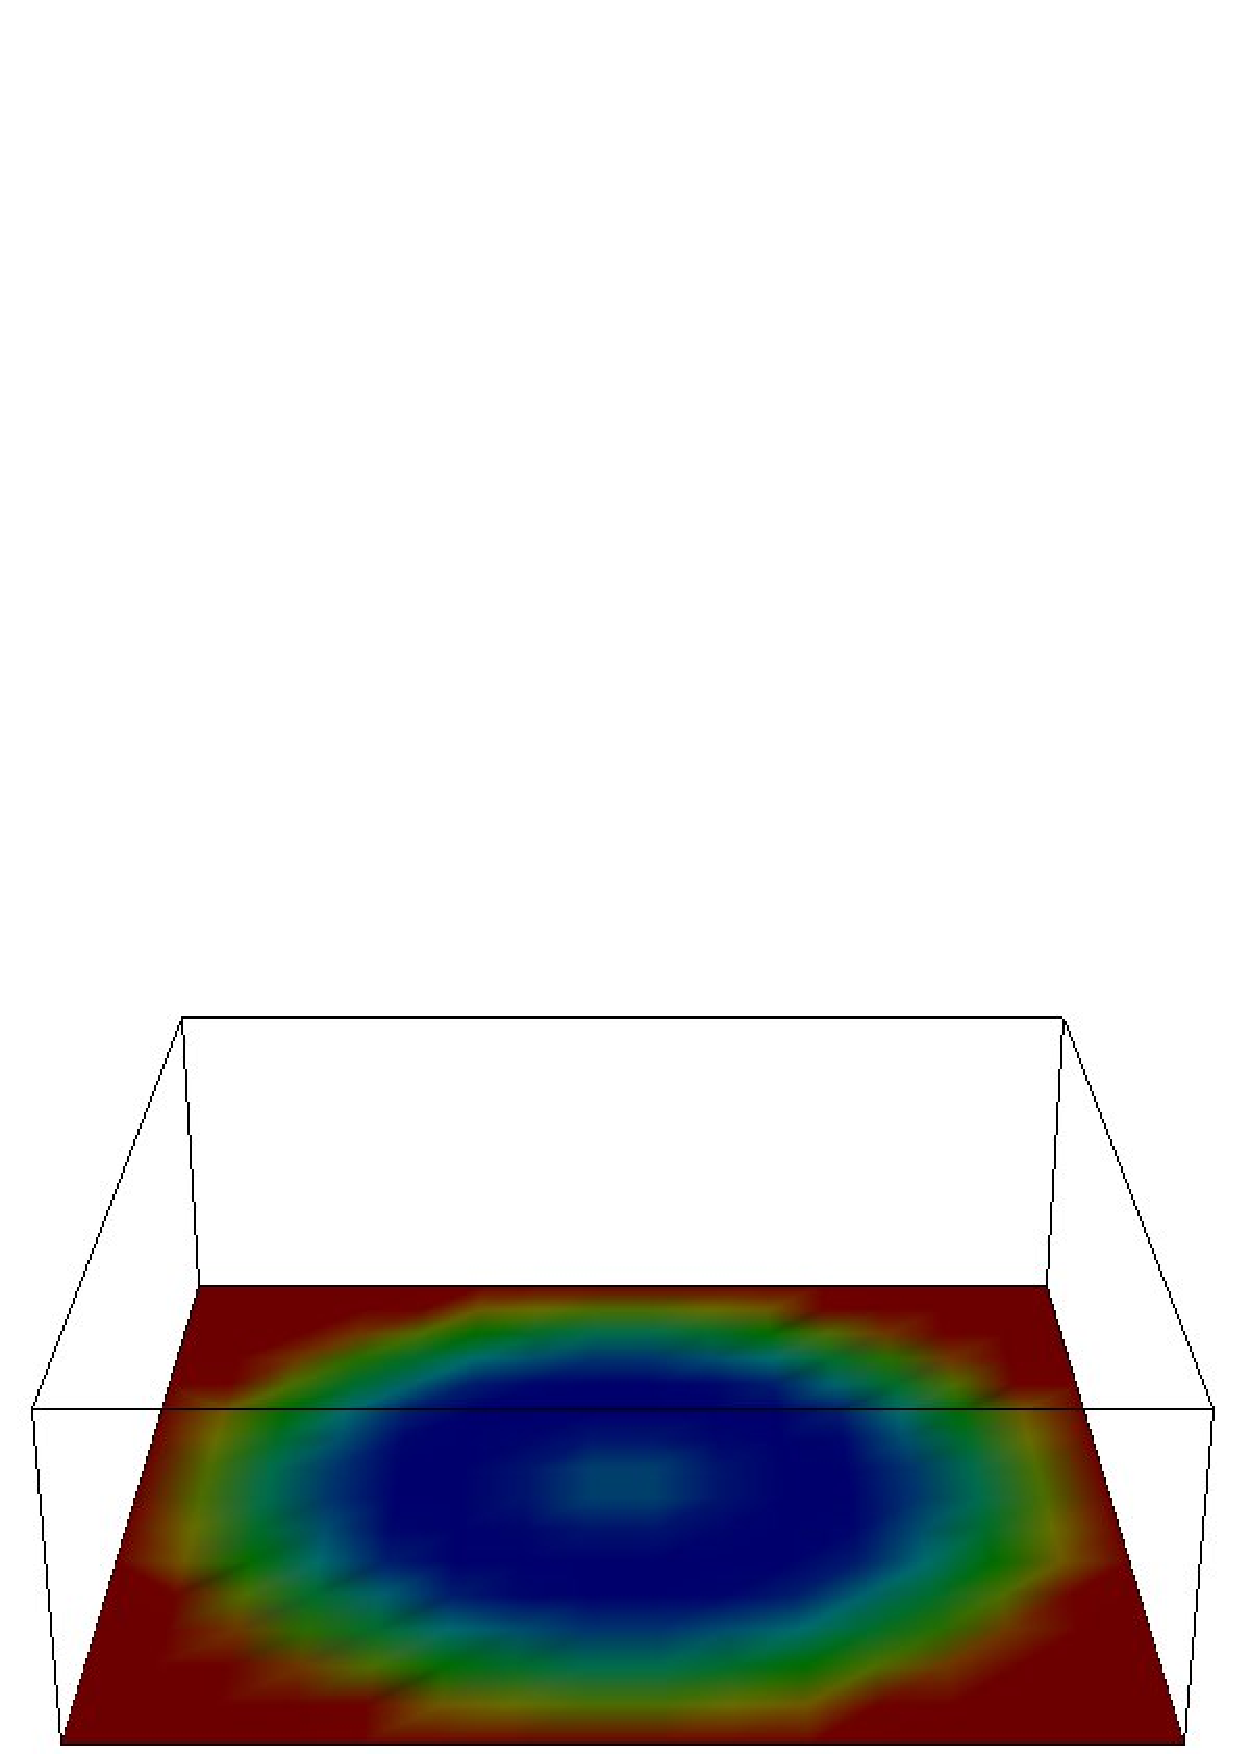
\includegraphics[width=40mm]{figures/MapOnPlane}
\end{center}
\caption{Surface map on a plane}
\label{fig:maponplane.1}
\end{figure}

\section{\MapOnClip class}
\begin{classdesc}{MapOnClip}{scene, data_collector, transform, lut = None}
A \MapOnClip object show a scalar field by color on a given clip.
\end{classdesc}

The following is a sample code using the \MapOnClip class. 
\fig{fig:maponclip.1} shows the corresponding output. 
\verbatiminput{../examples/drivermaponclip.py}

\begin{figure}[ht]
\begin{center}
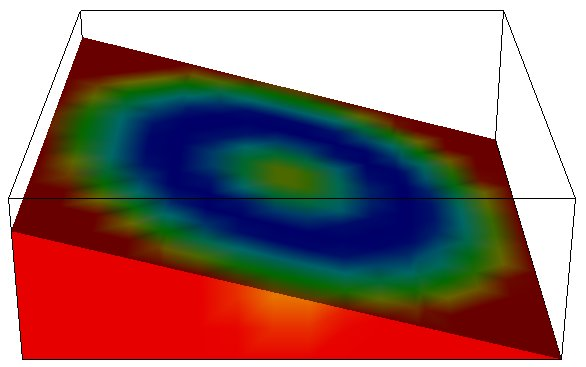
\includegraphics[width=40mm]{figures/MapOnClip}
\end{center}
\caption{Surface map on a clip}
\label{fig:maponclip.1}
\end{figure}

\section{\MapOnScalarClip class}
\begin{classdesc}{MapOnScalarClip}{scene, data_collector, lut = None}
A \MapOnScalarClip object show a scalar field by color on a given scalar clip.
\end{classdesc}

The following is a sample code using the \MapOnScalarClip class.
\fig{fig:maponscalarclip.1} shows the corresponding output.
\verbatiminput{../examples/drivermaponscalarclip.py}

\begin{figure}[ht]
\begin{center}
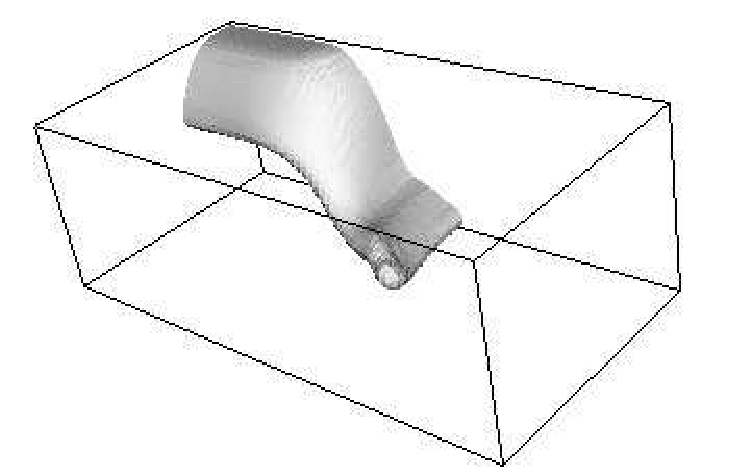
\includegraphics[width=40mm]{figures/MapOnScalarClip}
\end{center}
\caption{Surface map on a scalar clip}
\label{fig:maponscalarclip.1}
\end{figure}

\section{\Arrows class}
\begin{classdesc}{Arrows}{scene, data_collector, lut = None}
A \Arrows object shows a vector field by arrows.
\end{classdesc}

The following are the methods available:
\begin{methoddesc}[Arrows]{setVectorMode}{vector_mode}
Set the arrows vector mode.
\end{methoddesc}

\begin{methoddesc}[Arrows]{setScaleMode}{scale_mode}
Set the arrows scale mode.
\end{methoddesc}

\begin{methoddesc}[Arrows]{setScaleFactor}{scale_factor}
Set the arrows scale factor.
\end{methoddesc}

\begin{methoddesc}[Arrows]{setColorMode}{color_mode}
Set the arrows color mode.
\end{methoddesc}

The following is a sample code using the \Arrows class. 
\fig{fig:arrows.1} shows the corresponding output. 
\verbatiminput{../examples/driverarrows.py}

\begin{figure}[ht]
\begin{center}
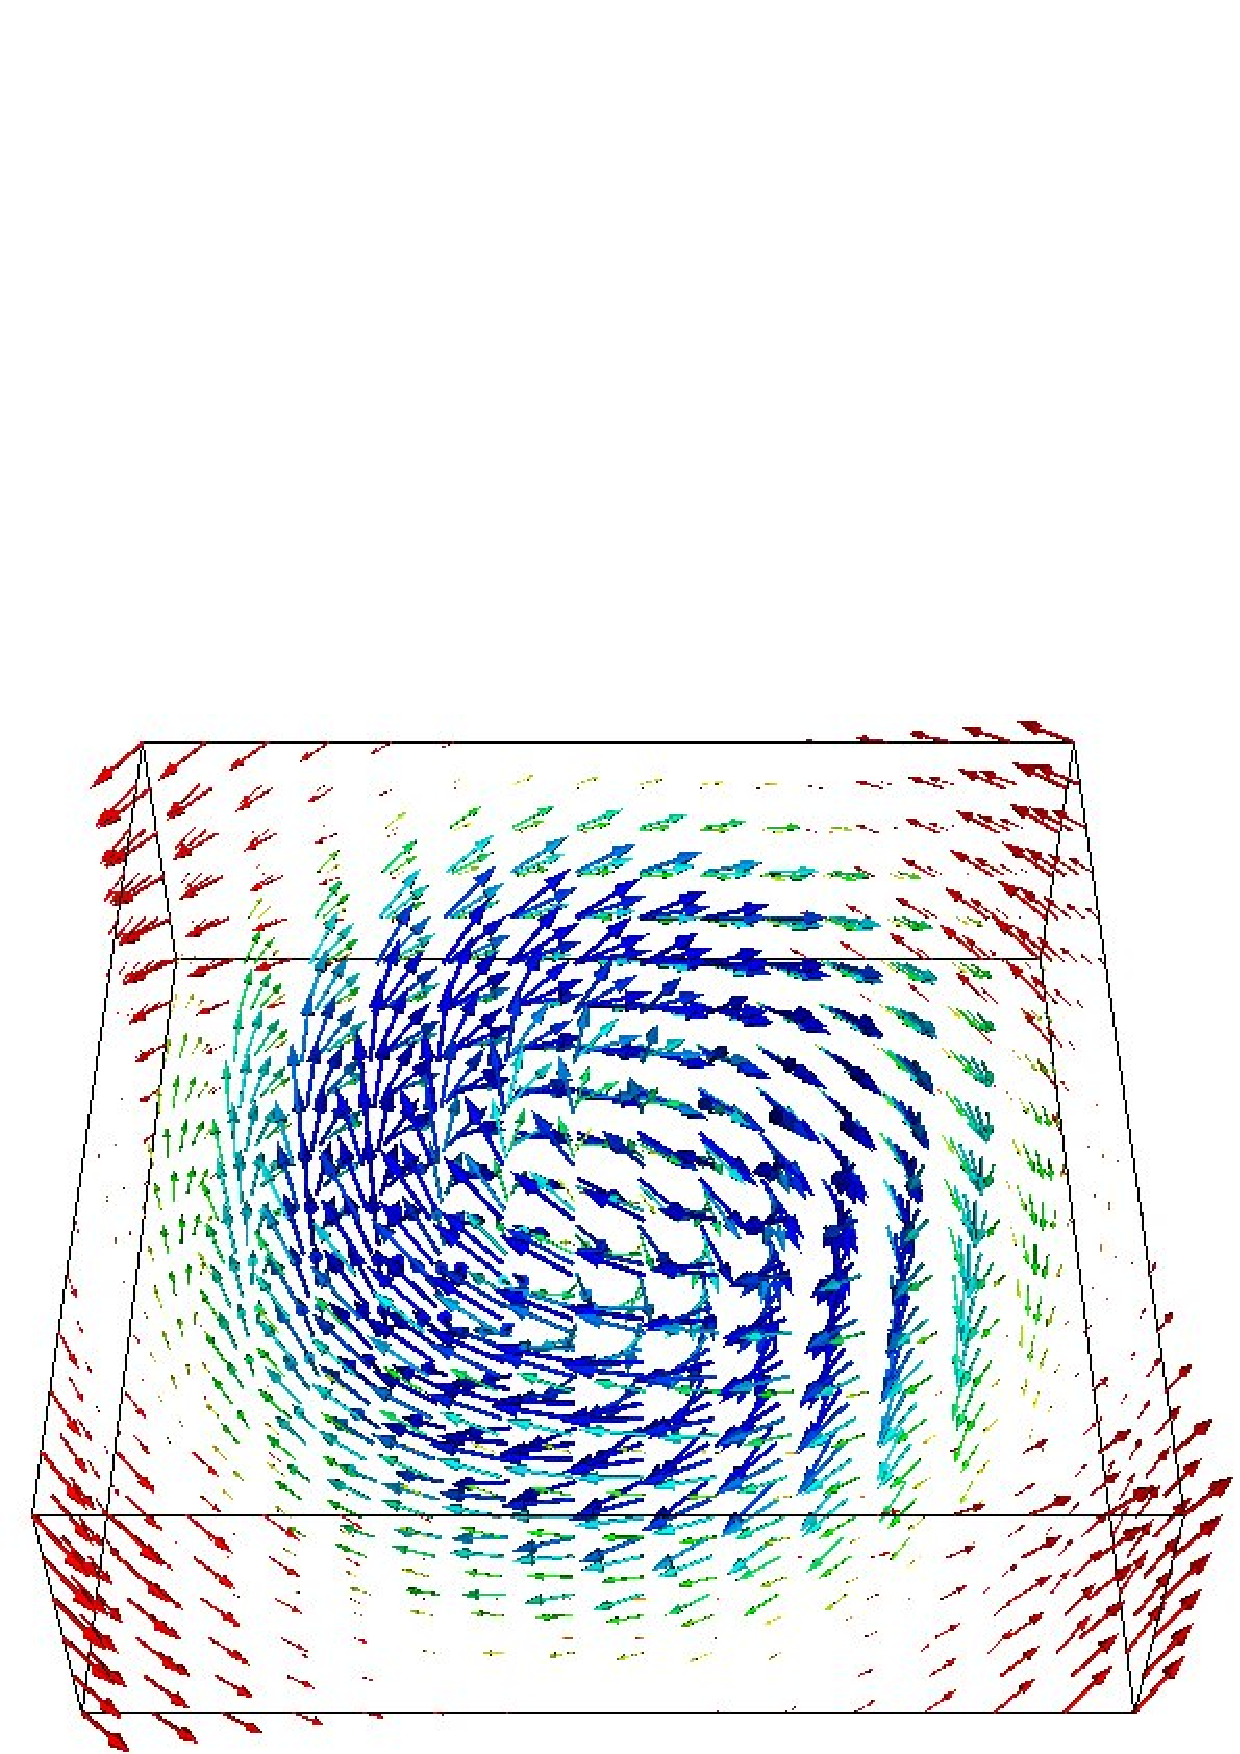
\includegraphics[width=40mm]{figures/Arrows}
\end{center}
\caption{Arrows}
\label{fig:arrows.1}
\end{figure}

\section{\ArrowsOnPlane class}
\begin{classdesc}{ArrowsOnPlane}{scene, data_collector, transform, lut = None}
A \ArrowsOnPlane object shows a vector field by arrows on a given plane.
\end{classdesc}

The following is a sample code using the \ArrowsOnPlane class. 
\fig{fig:arrowsonplane.1} shows the corresponding output. 
\verbatiminput{../examples/driverarrowsonplane.py}

\begin{figure}[ht]
\begin{center}
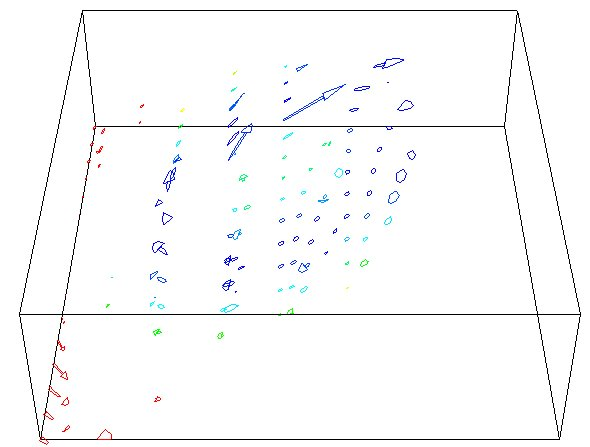
\includegraphics[width=40mm]{figures/ArrowsOnPlane}
\end{center}
\caption{Arrows on a plane}
\label{fig:arrowsonplane.1}
\end{figure}

\section{\ArrowsOnClip class}
\begin{classdesc}{ArrowsOnClip}{scene, data_collector, transform, lut = None}
A \ArrowsOnClip object shows a vector field by arrows on a given clip.
\end{classdesc}

The following is a sample code using the \ArrowsOnClip class.
\fig{fig:arrowsonclip.1} shows the corresponding output.
\verbatiminput{../examples/driverarrowsonclip.py}

\begin{figure}[ht]
\begin{center}
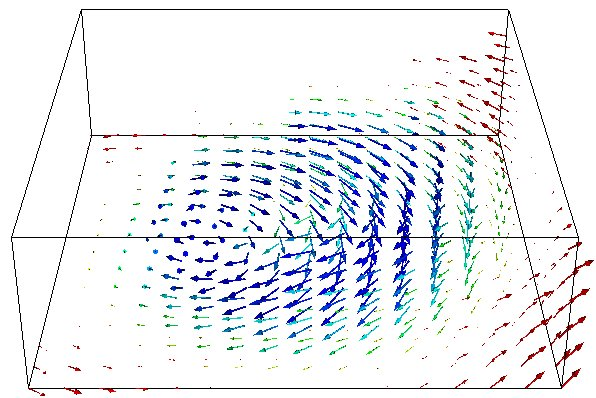
\includegraphics[width=40mm]{figures/ArrowsOnClip}
\end{center}
\caption{Arrows on a clip}
\label{fig:arrowsonclip.1}
\end{figure}


\section{\IsoSurface class}
\begin{classdesc}{IsoSurface}{scene, data_collector, lut = None}
An \IsoSurface object shows a scalar field for a given value by an isosurface.
\end{classdesc}

The following is the method available:

\begin{methoddesc}[IsoSurface]{setValue}{contour_number, value}
Set the contour number and value.
\end{methoddesc}

The following is a sample code using the \IsoSurface class.
\fig{fig:isosurface.1} shows the corresponding output.
\verbatiminput{../examples/driverisosurface.py}

\begin{figure}[ht]
\begin{center}
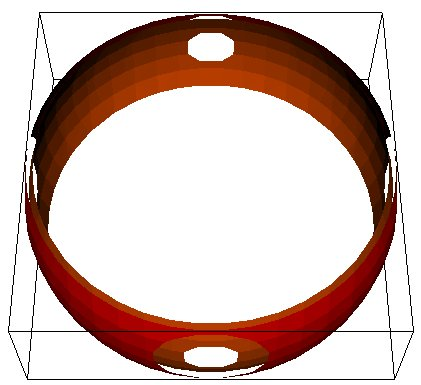
\includegraphics[width=40mm]{figures/IsoSurface}
\end{center}
\caption{IsoSurface}
\label{fig:isosurface.1}
\end{figure}

\section{\IsoSurfaceOnPlane class}
\begin{classdesc}{IsoSurfaceOnPlane}{scene, data_collector, transform, 
lut = None}
An \IsoSurfaceOnPlane object shows a scalar field for a given value 
by an isosurface on a given plane.
\end{classdesc}

The following is a sample code using the \IsoSurfaceOnPlane class.
\fig{fig:isosurfaceonplane.1} shows the corresponding output.
\verbatiminput{../examples/driverisosurfaceonplane.py}

\begin{figure}[ht]
\begin{center}
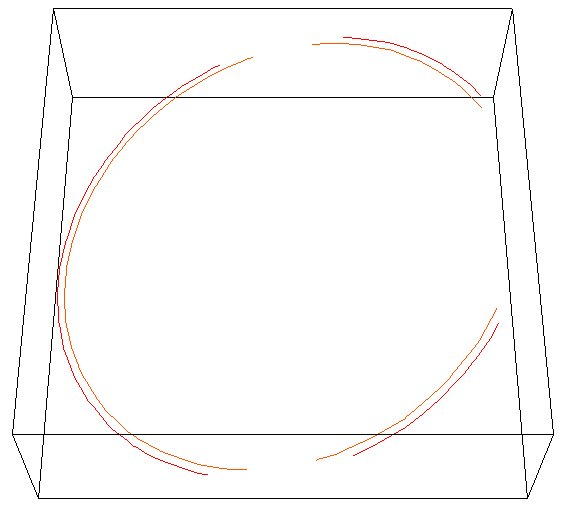
\includegraphics[width=40mm]{figures/IsoSurfaceOnPlane}
\end{center}
\caption{IsoSurface on a plane}
\label{fig:isosurfaceonplane.1}
\end{figure}

\section{\IsoSurfaceOnClip class}
\begin{classdesc}{IsoSurfaceOnClip}{scene, data_collector, transform, 
lut = None}
An \IsoSurfaceOnClip object shows a scalar field for a given value 
by an isosurface on a given clip.
\end{classdesc}

The following is a sample code using the \IsoSurfaceOnClip class.
\fig{fig:isosurfaceonclip.1} shows the corresponding output.
\verbatiminput{../examples/driverisosurfaceonclip.py}

\begin{figure}[ht]
\begin{center}
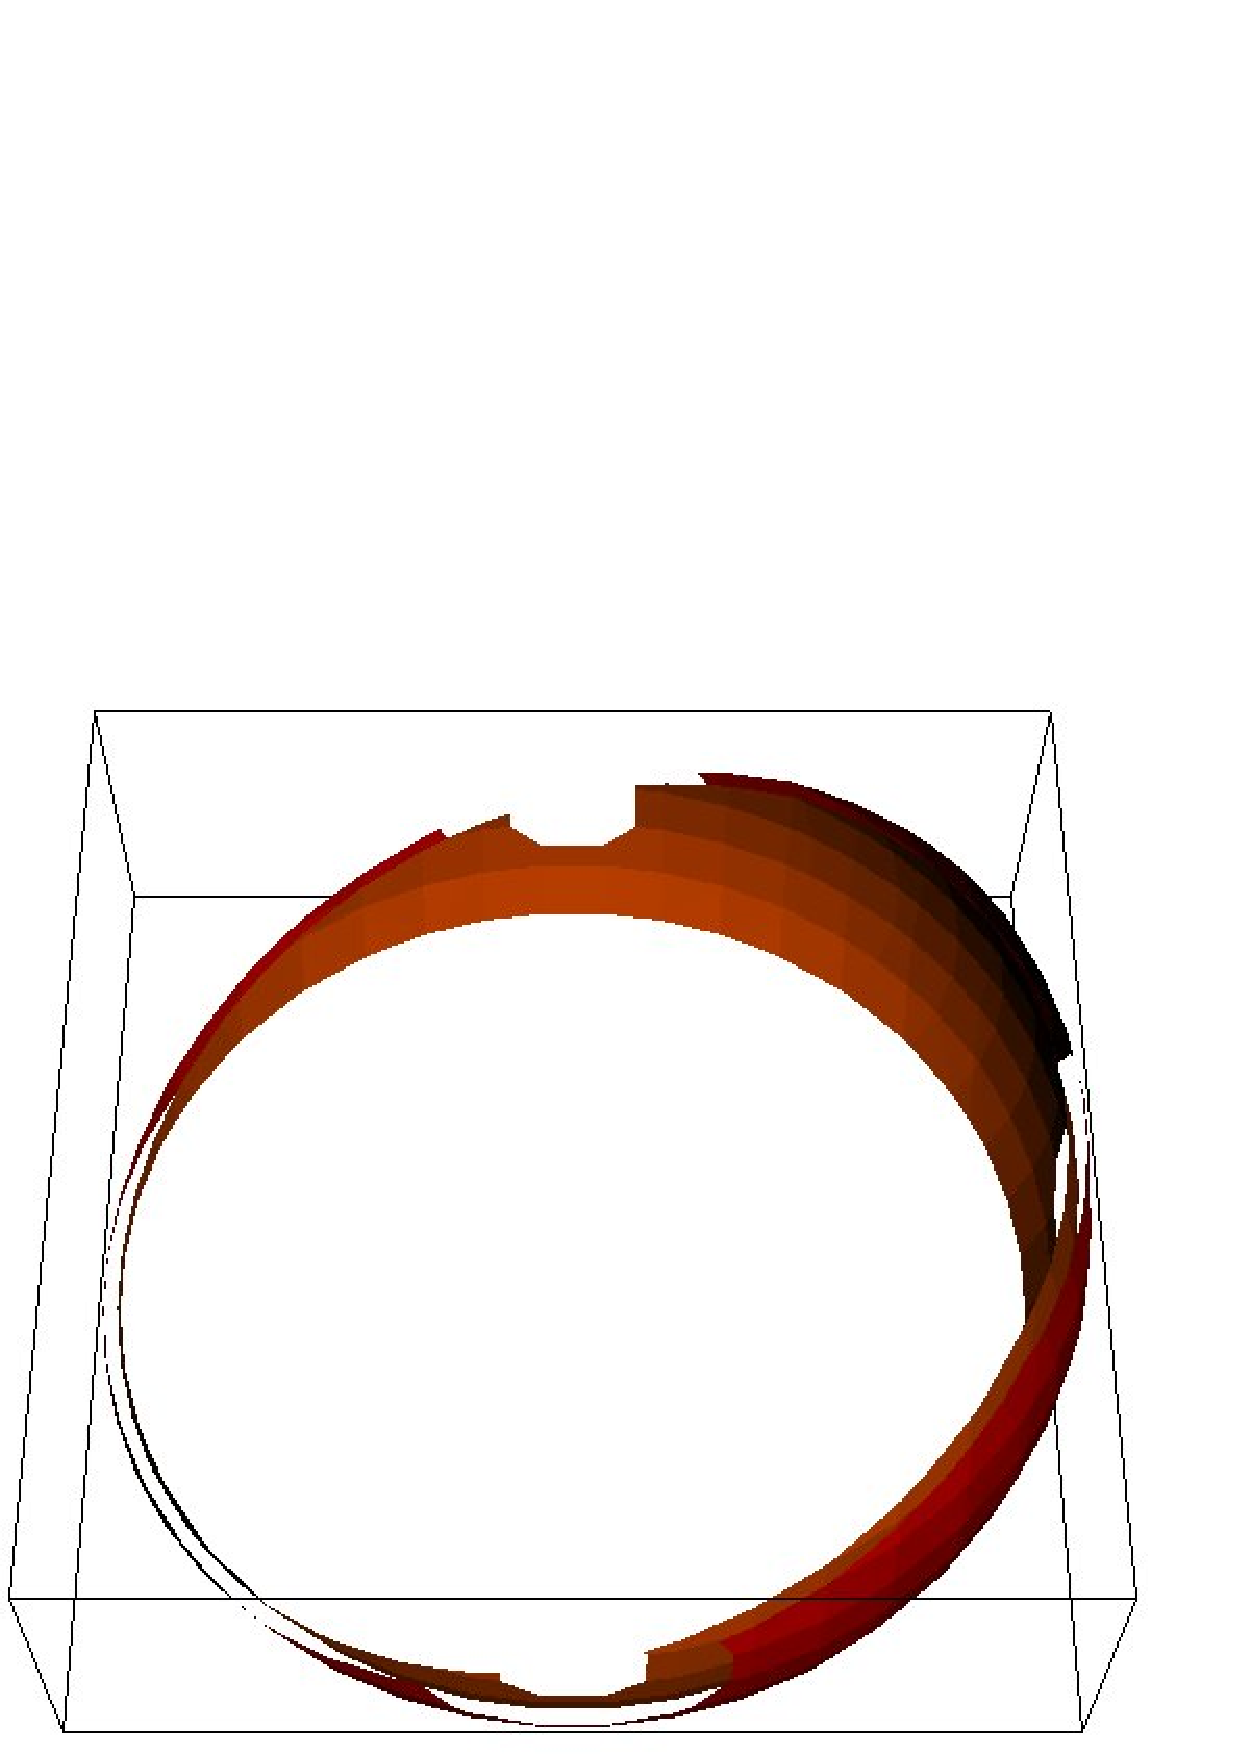
\includegraphics[width=40mm]{figures/IsoSurfaceOnClip}
\end{center}
\caption{IsoSurface on a clip}
\label{fig:isosurfaceonclip.1}
\end{figure}

\section{\Contour class}
\begin{classdesc}{Contour}{scene, data_collector, lut = None}
A \Contour object shows a scalar field contour surfaces.
\end{classdesc}

The following is the method available:
\begin{methoddesc}[Contour]{generateValues}{number_contours, min_range,
max_range}
Generate the specified number of contours within the specified range.
\end{methoddesc}

The following is a sample code using the \Contour class.
\fig{fig:contour.1} shows the corresponding output.
\verbatiminput{../examples/drivercontour.py}

\begin{figure}[ht]
\begin{center}
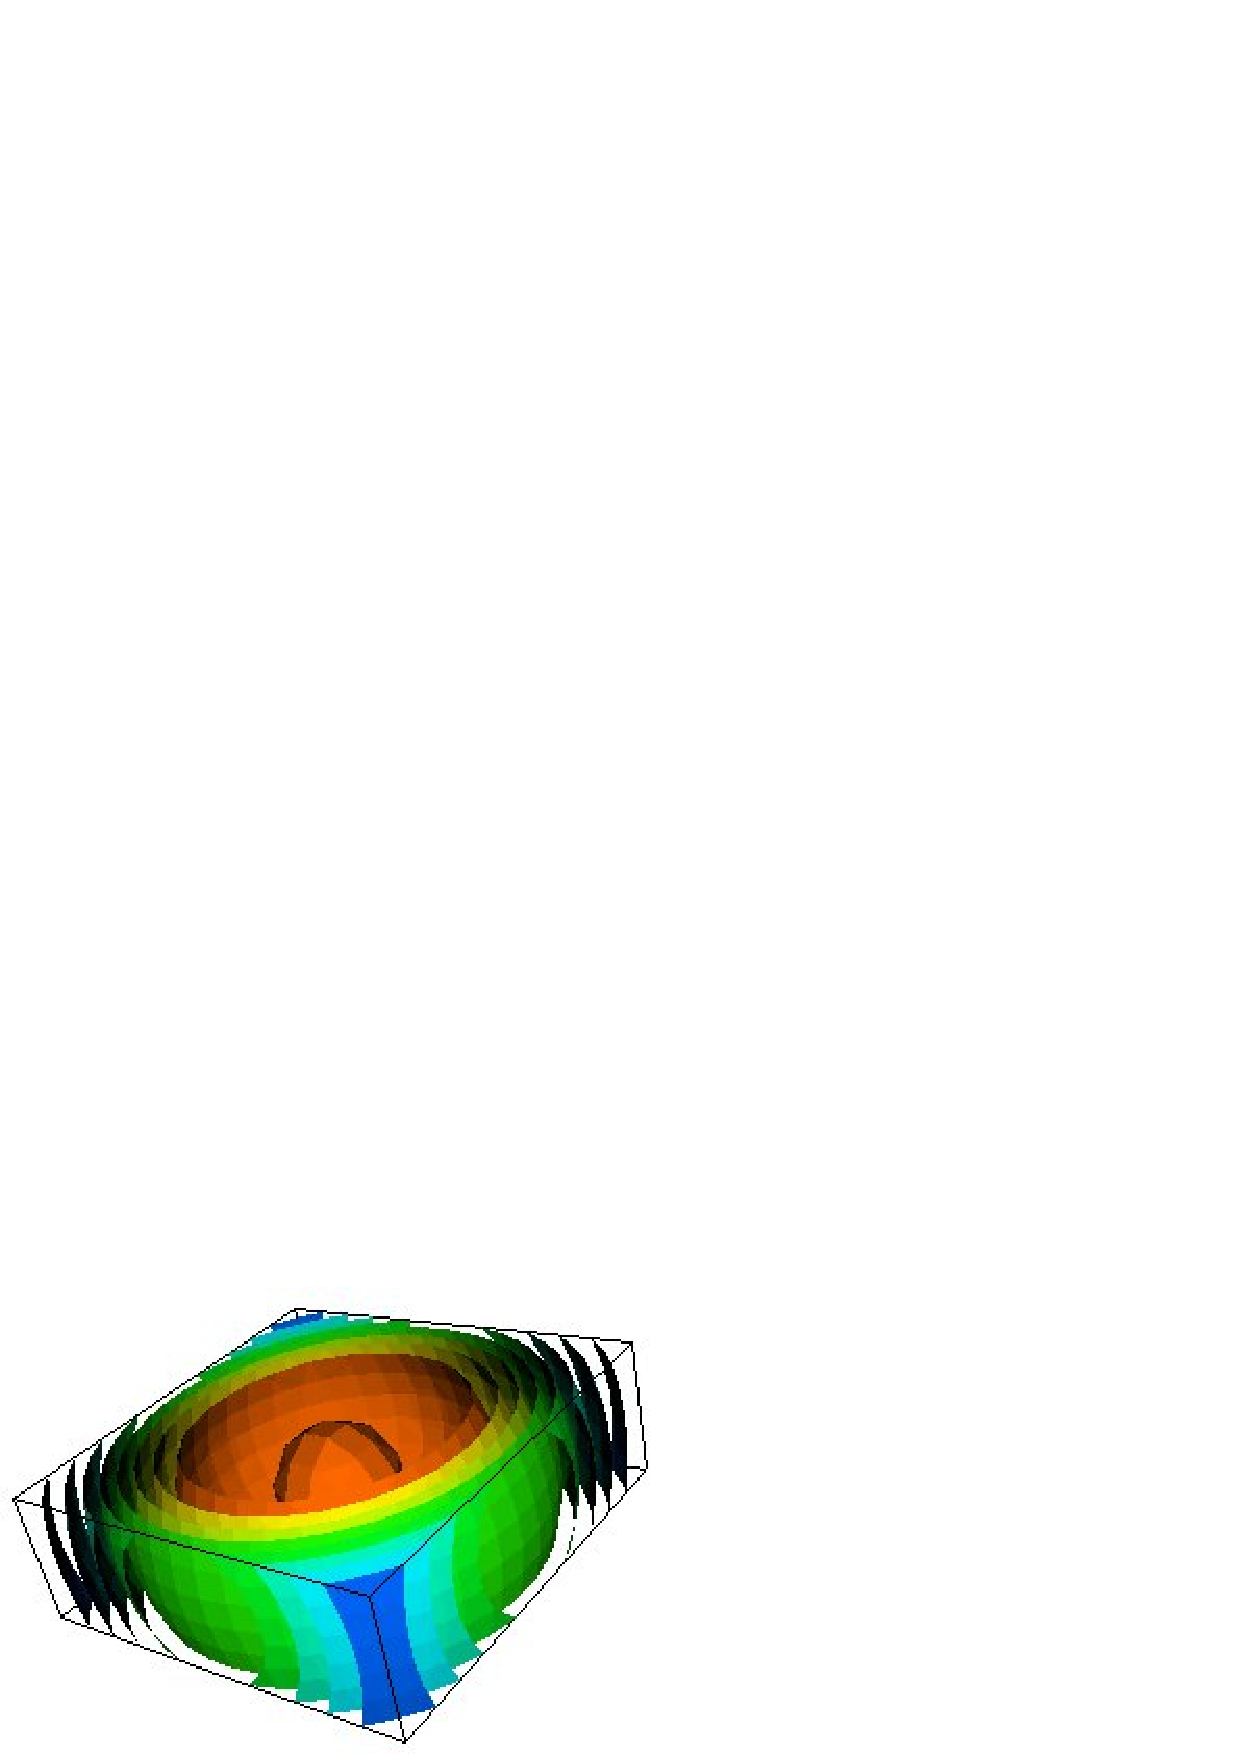
\includegraphics[width=40mm]{figures/Contour}
\end{center}
\caption{Contour}
\label{fig:contour.1}
\end{figure}

\section{\ContourOnPlane class}
\begin{classdesc}{ContourOnPlane}{scene, data_collector, transform, lut = None}
A \ContourOnPlane object shows a scalar field contour surfaces on a given plane.
\end{classdesc}

The following is a sample code using the \ContourOnPlane class.
\fig{fig:contouronplane.1} shows the corresponding output.
\verbatiminput{../examples/drivercontouronplane.py}

\begin{figure}[ht]
\begin{center}
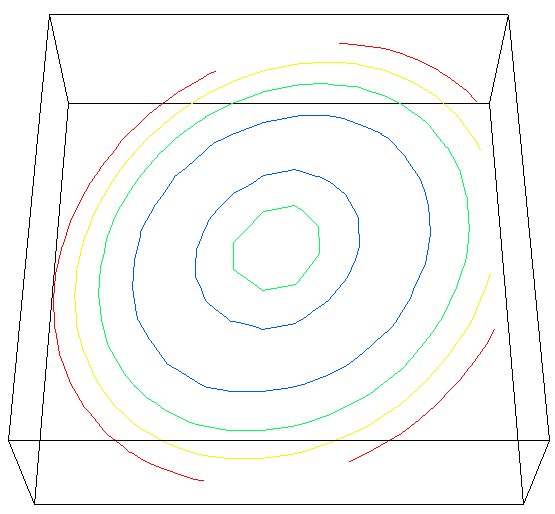
\includegraphics[width=40mm]{figures/ContourOnPlane}
\end{center}
\caption{Contour on a plane}
\label{fig:contouronplane.1}
\end{figure}

\section{\ContourOnClip class}
\begin{classdesc}{ContourOnClip}{scene, data_collector, transform, lut = None}
A \ContourOnClip object shows a scalar field contour surfaces on a given clip.
\end{classdesc}

The following is a sample code using the \ContourOnClip class.
\fig{fig:contouronclip.1} shows the corresponding output.
\verbatiminput{../examples/drivercontouronclip.py}

\begin{figure}[ht]
\begin{center}
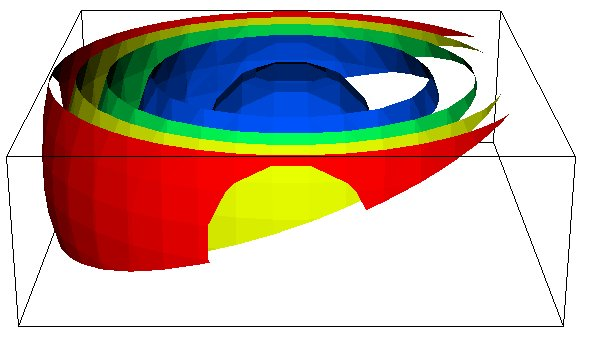
\includegraphics[width=40mm]{figures/ContourOnClip}
\end{center}
\caption{Contour on a clip}
\label{fig:contouronclip.1}
\end{figure}

\section{\TensorC class}
\begin{classdesc}{Tensor}{scene, data_collector, lut = None}
A \TensorC object shows a tensor field by ellipsoids.
\end{classdesc}

The following are the methods available:
\begin{methoddesc}[Tensor]{setThetaResolution}{resolution}
Set the number of points in the longitude direction.
\end{methoddesc}

\begin{methoddesc}[Tensor]{setPhiResolution}{resolution}
Set the number of points in the latitude direction.
\end{methoddesc}

\begin{methoddesc}[Tensor]{setScaleFactor}{scale_factor}
Set the tensor scale factor.
\end{methoddesc}

\begin{methoddesc}[Tensor]{setMaxScaleFactor}{max_scale_factor}
Set the maximum allowable scale factor.
\end{methoddesc}

The following is a sample code using the \TensorC class.
\fig{fig:tensor.1} shows the corresponding output.
\verbatiminput{../examples/drivertensor.py}

\begin{figure}[ht]
\begin{center}
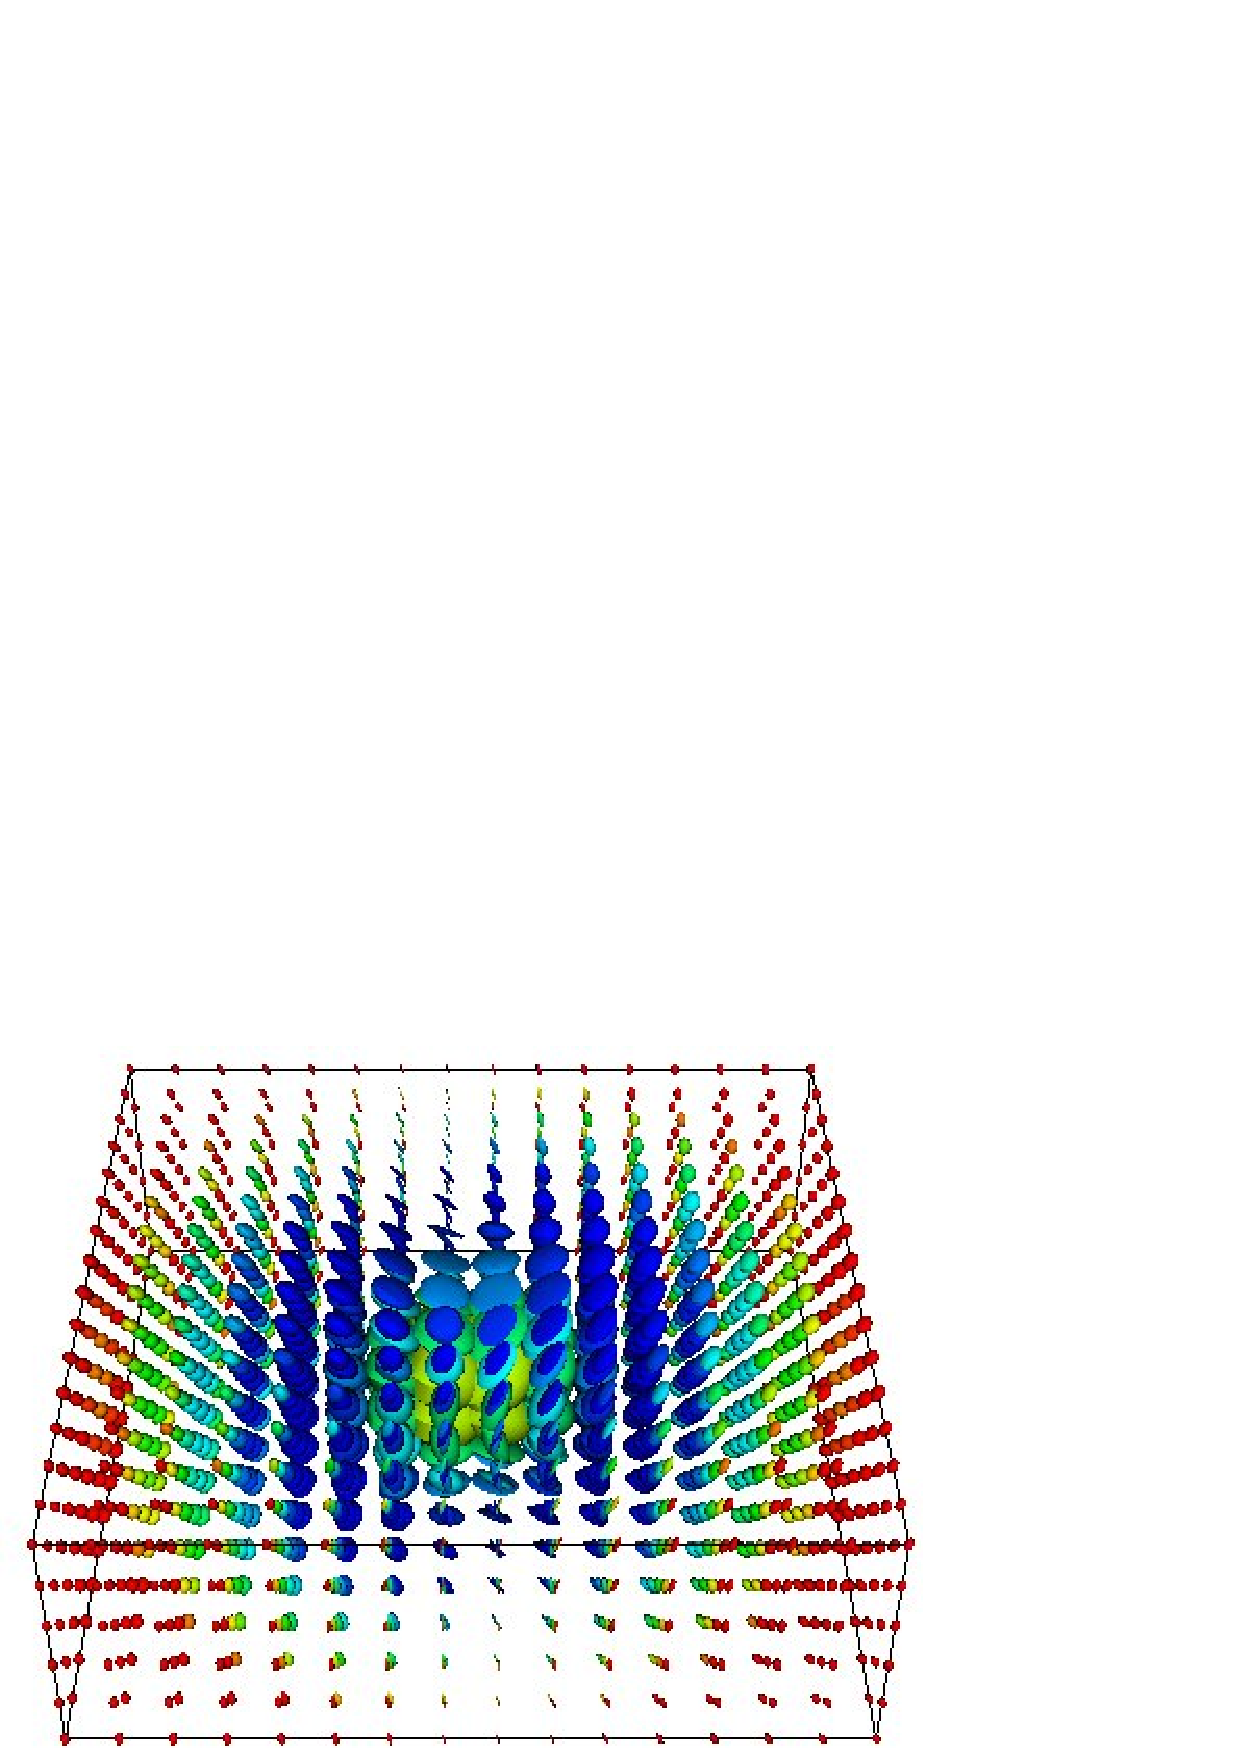
\includegraphics[width=40mm]{figures/Tensor}
\end{center}
\caption{Tensor}
\label{fig:tensor.1}
\end{figure}

\section{\TensorOnPlane class}
\begin{classdesc}{TensorOnPlane}{scene, data_collector, transform, lut = None}
A \TensorOnPlane object shows a tensor field by ellipsoids on a given plane.
\end{classdesc}

The following is a sample code using the \TensorOnPlane class.
\fig{fig:tensoronplane.1} shows the corresponding output.
\verbatiminput{../examples/drivertensoronplane.py}

\begin{figure}[ht]
\begin{center}
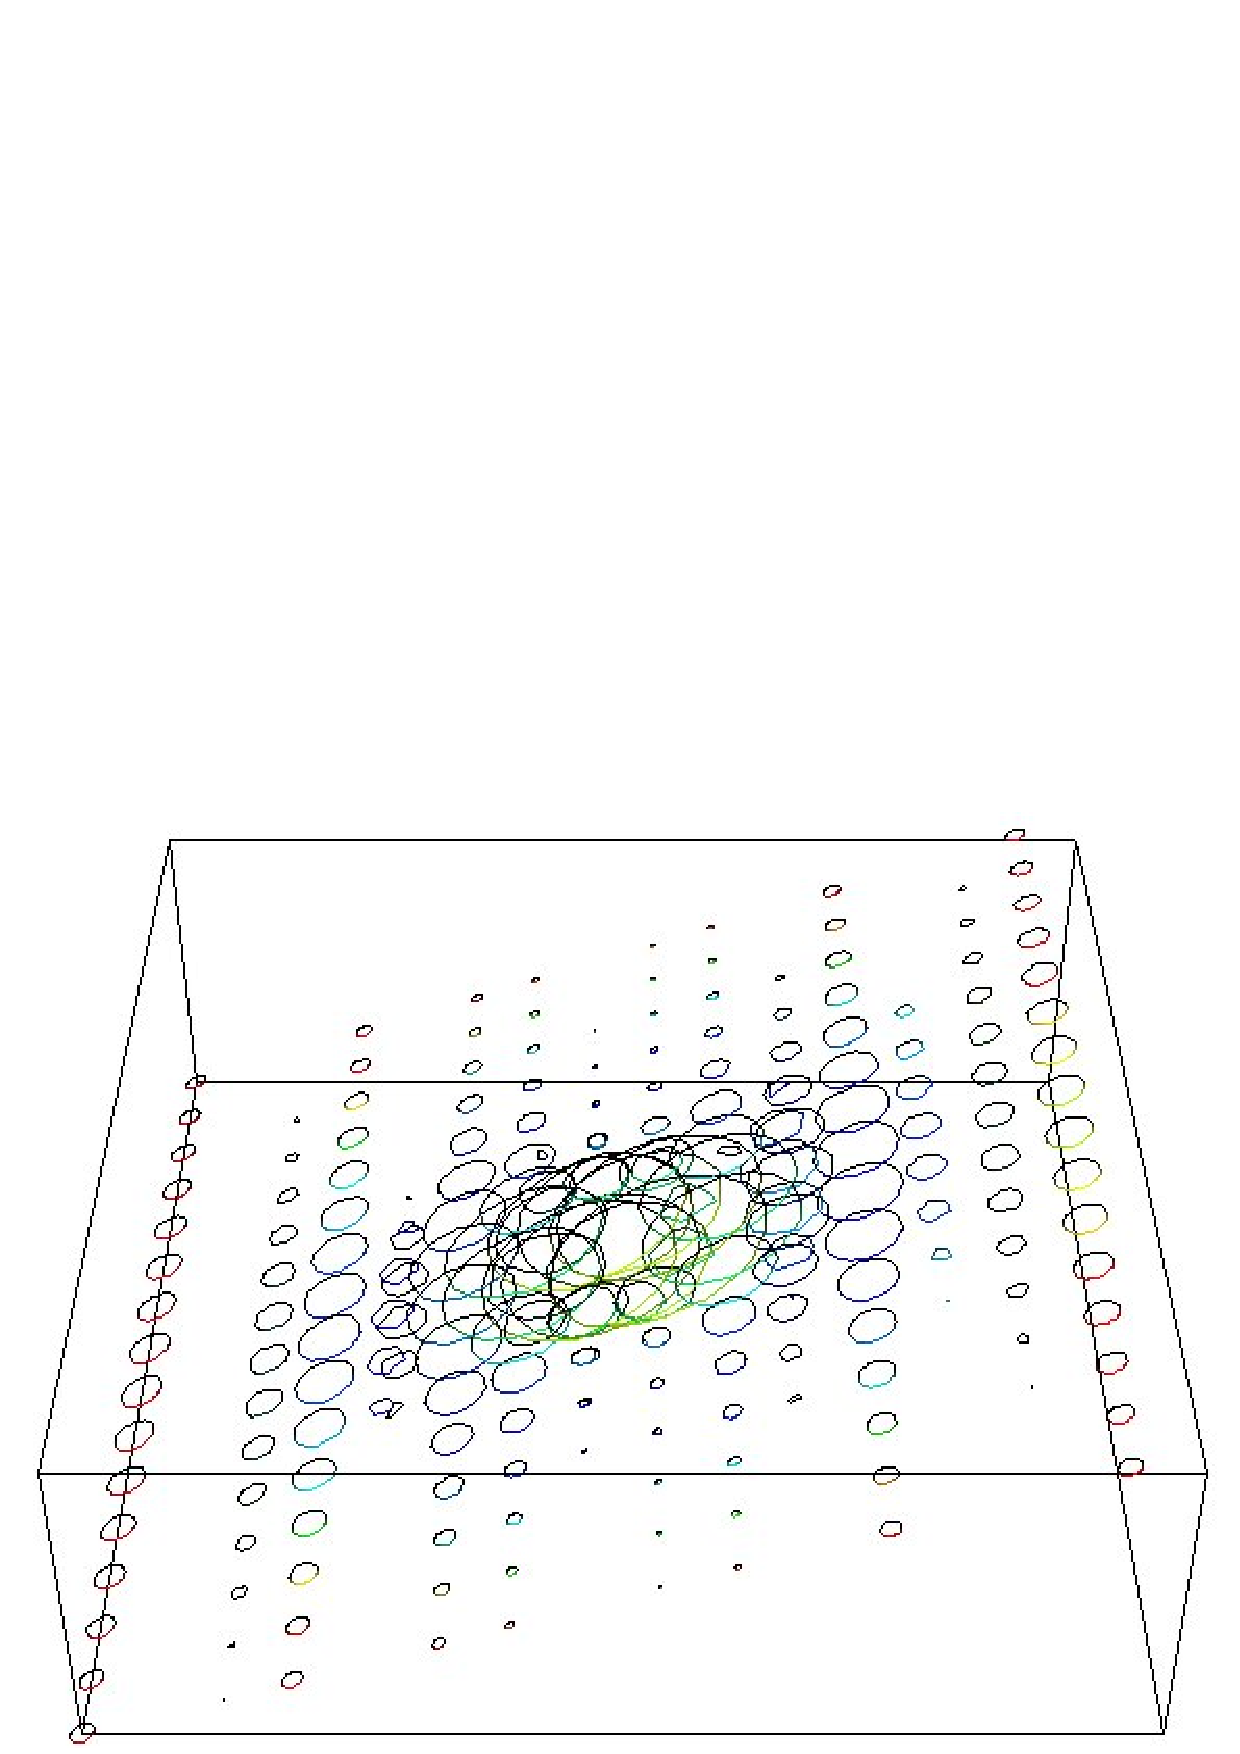
\includegraphics[width=40mm]{figures/TensorOnPlane}
\end{center}
\caption{Tensor on a plane}
\label{fig:tensoronplane.1}
\end{figure}

\section{\TensorOnClip class}
\begin{classdesc}{TensorOnClip}{scene, data_collector, transform, lut = None}
A \TensorOnClip object shows a tensor field by ellipsoids on a given clip.
\end{classdesc}

The following is a sample code using the \TensorOnClip class.
\fig{fig:tensoronclip.1} shows the corresponding output.
\verbatiminput{../examples/drivertensoronclip.py}

\begin{figure}[ht]
\begin{center}
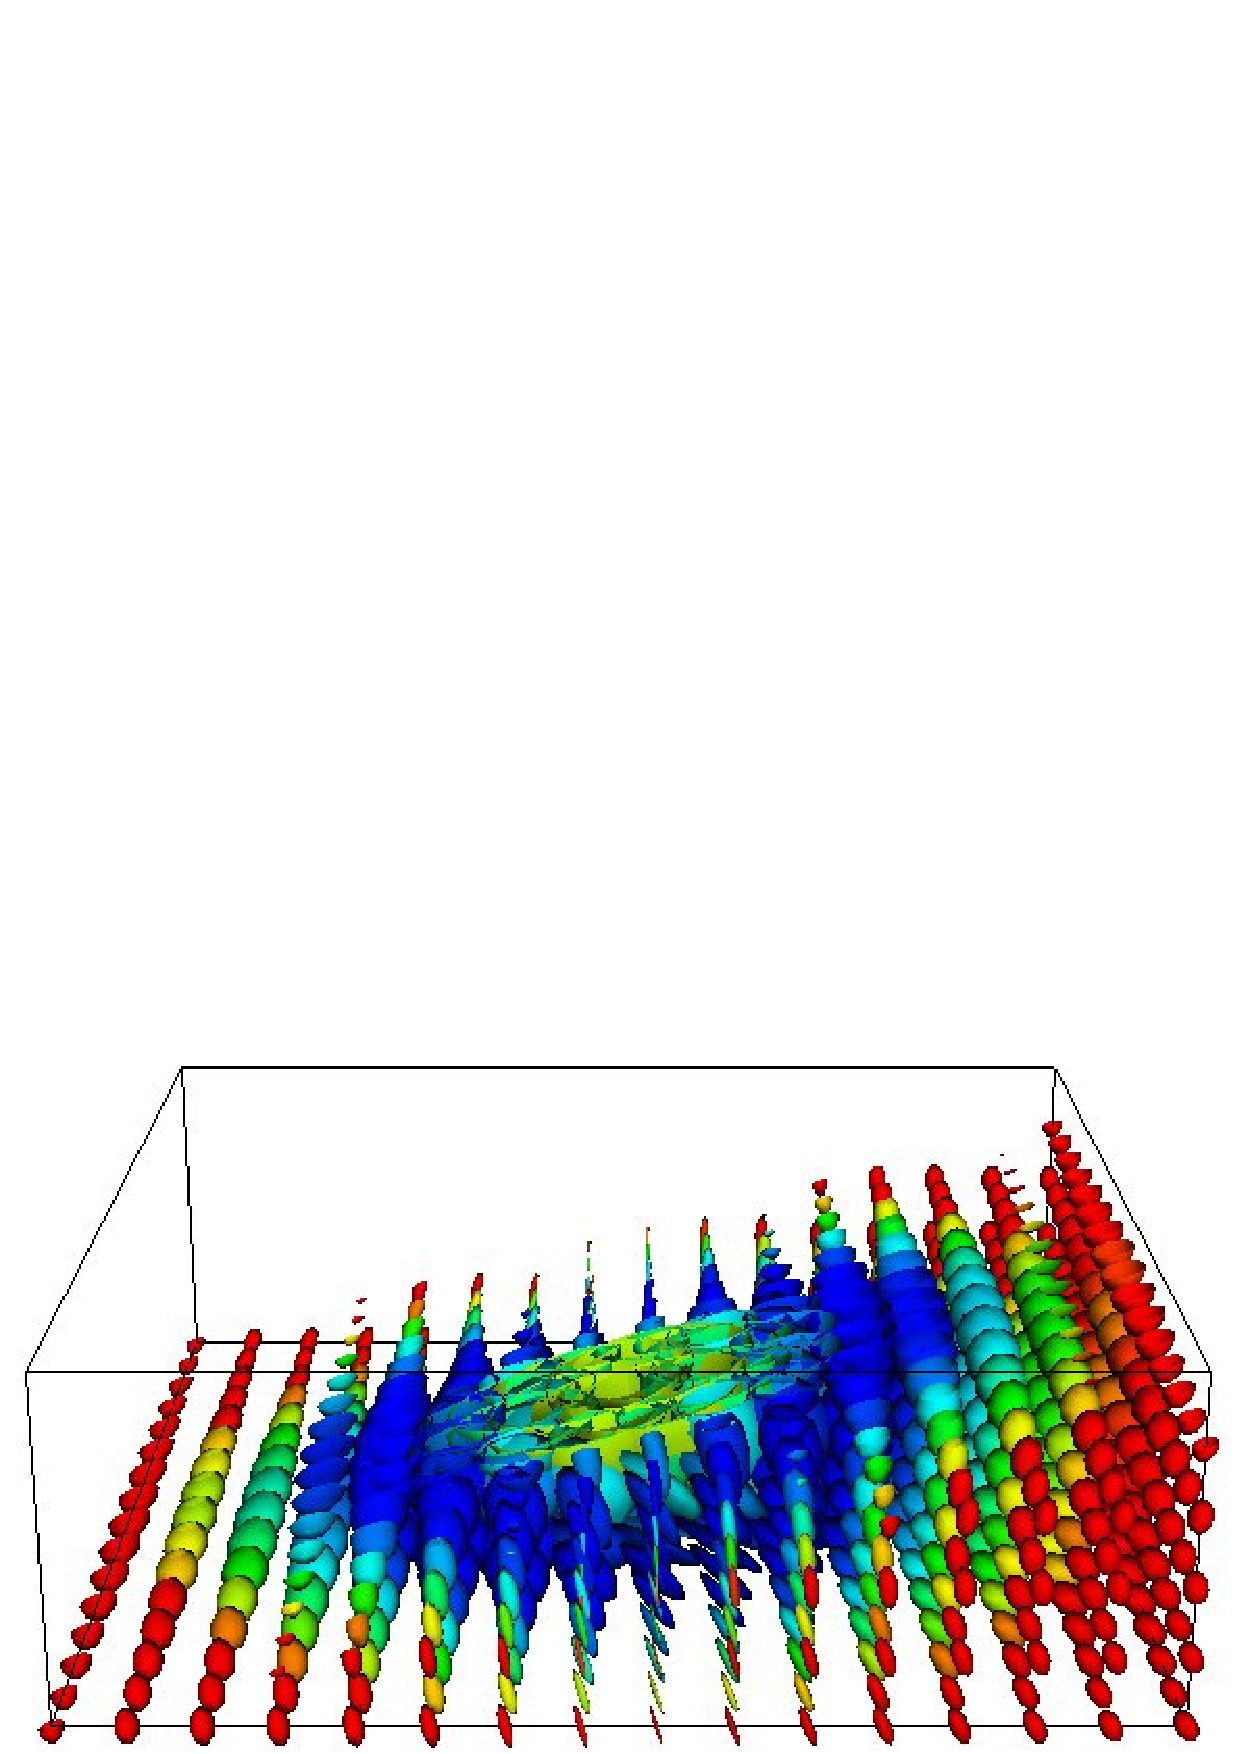
\includegraphics[width=40mm]{figures/TensorOnClip}
\end{center}
\caption{Tensor on a clip}
\label{fig:tensoronclip.1}
\end{figure}

\section{\StreamLines class}
\begin{classdesc}{StreamLines}{scene, data_collector, lut = None}
A \StreamLines object show the path of particles (within a specified cloud 
of points) in a vector field.
\end{classdesc}

The following are the methods available:
\begin{methoddesc}[StreamLines]{setCloudRadius}{radius}
Set the radius for the cloud of points.
\end{methoddesc}

\begin{methoddesc}[StreamLines]{setCenter}{position}
Set the center for the cloud of points.
\end{methoddesc}

\begin{methoddesc}[StreamLines]{setNumberOfPoints}{points}
Set the number of points to generate for the cloud of points.
\end{methoddesc}

\begin{methoddesc}[StreamLines]{setMaximumPropagationTime}{time}
Set the maximum length for the streamlines in unit of time.
\end{methoddesc}

\begin{methoddesc}[StreamLines]{setStreamLinesSize}{stream_lines_size}
Set the size of the steamlines.
\end{methoddesc}

\begin{methoddesc}[StreamLines]{setAccuracy}{accuracy}
Set the accuracy for the streamlines.
\end{methoddesc}

\begin{methoddesc}[StreamLines]{setIntegrationToBothDirections}{}
Set the integration to occur in both directions.
\end{methoddesc}

\begin{methoddesc}[StreamLines]{setTubeRadius}{radius}
Set the minimum radius of the tube.
\end{methoddesc}

\begin{methoddesc}[StreamLines]{setNumberOfSides}{sides}
Set the number of sides for the tube.
\end{methoddesc}

\begin{methoddesc}[StreamLines]{setVaryRadiusByVector}{}
Set the variation of the tube radius with vector data.
\end{methoddesc}

The following is a sample code using the \StreamLines class.
\fig{fig:streamlines.1} shows the corresponding output.
\verbatiminput{../examples/driverstreamlines.py}

\begin{figure}[ht]
\begin{center}
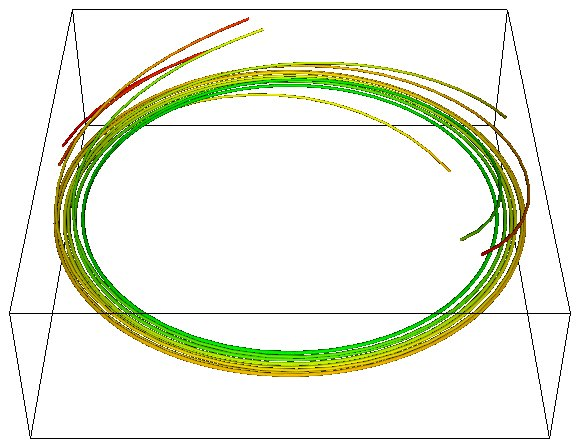
\includegraphics[width=40mm]{figures/StreamLines}
\end{center}
\caption{StreamLines}
\label{fig:streamlines.1}
\end{figure}

\section{\Carpet class}
\begin{classdesc}{Carpet}{scene, data_collector, transform, lut = None, 
deform = None}
A \Carpet object shows a scalar/vector field as a plane deformated along 
the plane normal.
\end{classdesc}

The following is the method available:
\begin{methoddesc}[Carpet]{setScaleFactor}{scale_factor}
Set the displancement scale factor.
\end{methoddesc}

The following is a sample code using the \Carpet class.
\fig{fig:carpet.1} shows the corresponding output.
\verbatiminput{../examples/drivercarpet.py}

\begin{figure}[ht]
\begin{center}
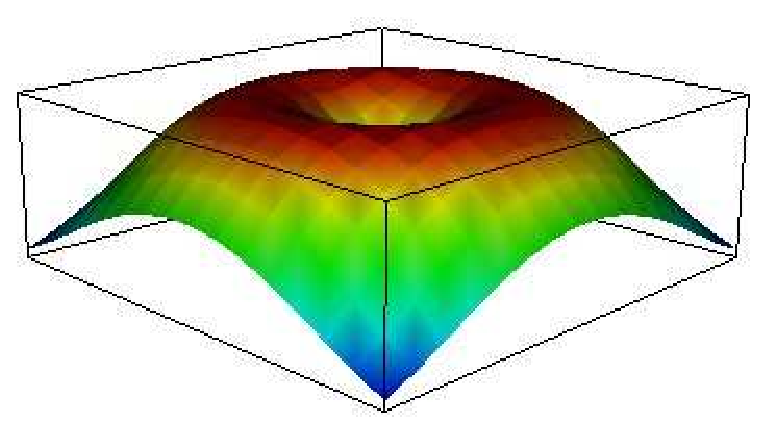
\includegraphics[width=40mm]{figures/Carpet}
\end{center}
\caption{Carpet}
\label{fig:carpet.1}
\end{figure}


\section{\Position class}
\begin{classdesc}{Position}{x_coor, y_coor, z_coor}
A \Position object defines the x, y and z coordinates of rendered object.
\end{classdesc}

\section{\Transform class}
\begin{classdesc}{Transform}{}
A \Transform object defines the orientation of rendered object.
\end{classdesc}

The following are some of the methods available:
\begin{methoddesc}[Transform]{translate}{x_offset, y_offset, z_offset}
Translate the rendered object along the x, y and z-axes.
\end{methoddesc}

\begin{methoddesc}[Transform]{rotateX}{angle}
Rotate the rendered object along the x-axis.
\end{methoddesc}

\begin{methoddesc}[Transform]{rotateY}{angle}
Rotate the rendered object along the y-axis.
\end{methoddesc}

\begin{methoddesc}[Transform]{rotateZ}{angle}
Rotate the rendered object along the z-axis.
\end{methoddesc}

\begin{methoddesc}[Transform]{xyPlane}{offset = 0}
Set the plane orthogonal to the z-axis.
\end{methoddesc}

\begin{methoddesc}[Transform]{yzPlane}{offset = 0}
Set the plane orthogonal to the x-axis.
\end{methoddesc}

\begin{methoddesc}[Transform]{xzPlane}{offset = 0}
Set the plane orthogonal to the y-axis.
\end{methoddesc}

\section{\Style class}
\begin{classdesc}{Style}{}
A \Style object defines the style of text.
\end{classdesc}

The following are the methods available:
\begin{methoddesc}[Style]{setFontFamily}{family}
Set the font family (i.e. Times)
\end{methoddesc}

\begin{methoddesc}[Style]{boldOn}{}
Bold the text.
\end{methoddesc}

\begin{methoddesc}[Style]{italicOn}{}
Italize the text.
\end{methoddesc}

\begin{methoddesc}[Style]{shadowOn}{}
Apply shadows on the text.
\end{methoddesc}

\begin{methoddesc}[Style]{setColor}{}
Set the text color.
\end{methoddesc}

\section{\BlueToRed class}
\begin{classdesc}{BlueToRed}{}
A \BlueToRed object defines a map spectrum from blue to red.
\end{classdesc}

\section{\RedToBlue class}
\begin{classdesc}{RedToBlue}{}
A \RedToBlue object defines a map spectrum from red to blue.
\end{classdesc}

\section{\Plane class}
The following are the methods available:
\begin{methoddesc}[Plane]{setPlaneOrigin}{position}
Set the plane origin
\end{methoddesc}

\begin{methoddesc}[Plane]{setPlaneNormal}{position}
Set the plane normal
\end{methoddesc}

\begin{methoddesc}[Plane]{setValue}{clipping_value}
Set the clipping value
\end{methoddesc}

\begin{methoddesc}[Plane]{setInsideOutOn}{}
Set the clipping to inside out
\end{methoddesc}

\begin{methoddesc}[Plane]{setInsideOutOff}{}
Disable the inside out clipping
\end{methoddesc}

\section{Additional Notes}
The following is a sample code rendering multiple planes. 
\fig{fig:multipleplanes.1} shows the corresponding output.
\verbatiminput{../examples/drivermultipleplanes.py}

\begin{figure}[ht]
\begin{center}
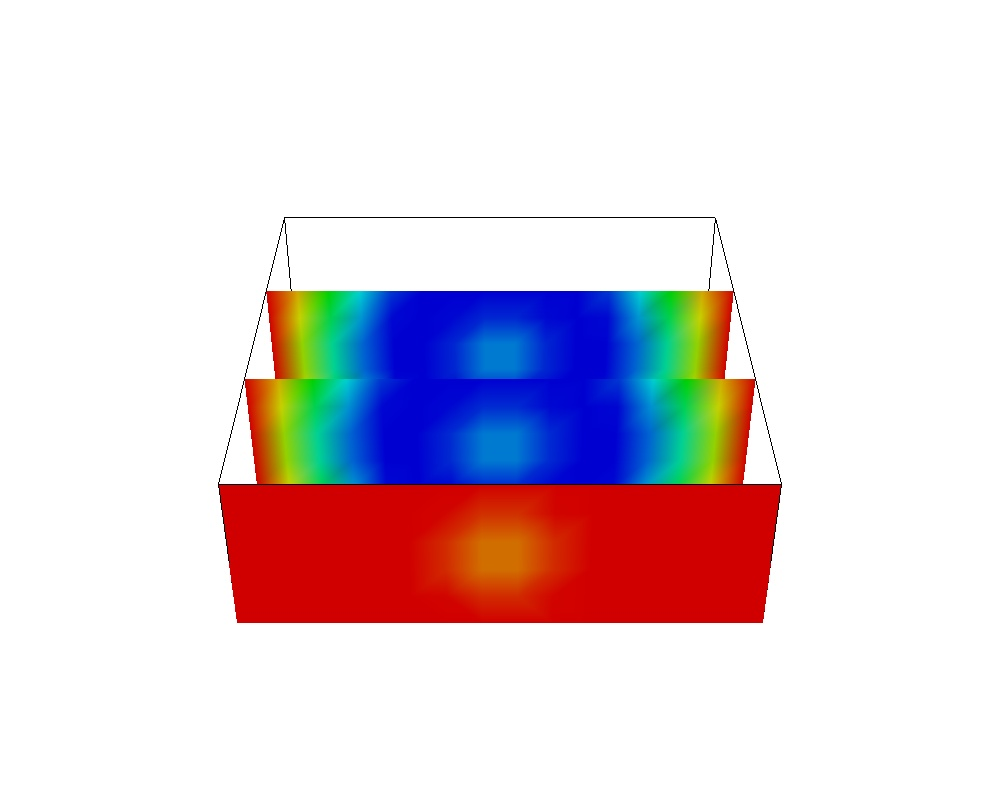
\includegraphics[width=60mm]{figures/MultiplePlanes}
\end{center}
\caption{Multiple planes}
\label{fig:multipleplanes.1}
\end{figure}

The following is a sample code rendering multiple cuts.
\verbatiminput{../examples/drivermultiplecuts.py}


The following is a sample code rendering multiple reads from multiple files.
\verbatiminput{../examples/drivermultiplereads.py}

